\subsection{Variando el porcentaje de modificación del grafo causal}\label{exp1}

Se realiza una serie de experimentos donde se busca mostrar el comportamiento 
del método propuesto sobre subgrafos del grafo causal verdadero. Estos subgrafos son generados a partir del $\mathcal{D}$, alterándolo a diferentes niveles.

\subsubsection{Configuración experimental}

\begin{itemize}
    \item El espacio de estados es discreto, es decir, el agente puede
    obtener las variables $\mathcal{X}$ directamente del ambiente.
    \item Se prueba modificando el grafo $\mathcal{D}$ para obtener a los
    grafos $\mathcal{D'}$ y $\mathcal{D''}$ en tres niveles. El porcentaje de nivel de cambio se representa con el parámetro $p_{mod}$.
    Para cada nivel, el subgrafo $\mathcal{D'}$ se genera al remover un porcentaje $p_{mod}$ de las aristas en el grafo $\mathcal{D}$. Para producir $\mathcal{D''}$ se elimina $p_{mod}$ de las aristas y después, de la mitad de conexiones perdidas, se crean nuevas diferentes a las iniciales.
    \begin{itemize}
        \item Nivel bajo de modificación, $p_{mod} = 25 \%$.
        \item Nivel medio de modificación. $p_{mod} = 50 \%$.
        \item Nivel alto de modificación. $p_{mod} = 75 \%$
    \end{itemize}
    \item Se examina sobre los tres tipos de estructuras posibles: uno-a-uno, 
    causa común y efecto común. 
    \item Se prueba sobre ambientes deterministas y estocásticos.
    
    \item La tasa de exploración está dada por un $\delta = 0.5$ lo que indica que aproximadamente a mitad del entrenamiento la probabilidad de explotación alcanza su máximo valor.
\end{itemize}

\subsubsection{Objetivo}

Determinar si la información provista por un modelo
incompleto o parcialmente incorrecto ayuda y no
afecta negativamente el desempeño del algoritmo de RL.

\subsubsection{Hipótesis}

Dado que la información del modelo causal solo guía la selección
de acciones durante la exploración, entonces un grafo con escasos
datos correctos sigue siendo mejor que una búsqueda aleatoria. 
% En el
% peor caso, el algoritmo se comportaría como el método sin información adicional.


\subsubsection{Resultados}

Para comparar el desempeño de los distintos algoritmos propuestos
para todas las diferentes configuraciones del experimento
se evalúa la medida \textit{average} descrita anteriormente.
De manera gráfica se puede ver el desempeño de los algoritmos
para los diferentes valores de $p_{mod}$ y tipo de ambiente en las Figuras \ref{fig:low-mod-det}, \ref{fig:low-mod-sto}, \ref{fig:med-mod-det}, \ref{fig:med-mod-sto},  \ref{fig:high-mod-det} y \ref{fig:high-mod-sto}.

De acuerdo con las Figuras \ref{fig:low-mod-det}-\ref{fig:high-mod-sto}
en la mayoría de los casos los algoritmos que utilizan conocimiento del grafo inician con una recompensa mayor y se estabilizan más rápido que el algoritmo Q-learning
sin información adicional en ambientes con transiciones deterministas y estocásticas. Para el caso donde $p_{mod} = 25$, los algoritmos con información incompleta e incorrecta parecen 
comportarse de manera muy similar. Esto puede ser debido 
a que la tasa de alteración del grafo es muy baja y  a que $N$ no toma
valores muy grandes, por lo que hay muy poca diferencia entre el grafo incompleto y el incorrecto. 
En el caso de $p_{mod} = 50$, se
puede notar que el desempeño de los algoritmos
con información incompleta e incorrecta se 
va moviendo en dirección a la curva del algoritmo
Q-learning sin información extra.
Finalmente, para $p_{mod} = 75$,  a pesar de haber modificado el grafo 
causal en un porcentaje bastante alto, la poca información que queda y es correcta sigue siendo suficiente para alcanzar una recompensa mayor mucho más rápido, donde al menos es más notable para las estructuras de tipo causa común y de efecto común.
Existe un comportamiento extraño en las tareas con una estructura del tipo uno a uno. Se puede ver que entre más crece el valor de $N$ los algoritmos que utilizan el grafo tienden a decrecer en dirección al punto de transición en el que la explotación llega a su máximo valor. Sin embargo, una vez que pasa ese punto, los algoritmos se siguen comportando de manera superior al algoritmo clásico.


Por otro lado, además de la colección de medidas en forma de curvas de aprendizaje, se propone hacer una comparación estadística de
los métodos. Para llevar a cabo esta última, se compara la recompensa promedio de los últimos $E$ episodios
de entrenamiento sobre los $M$ experimentos. Con esto, se 
puede obtener una muestra de tamaño $E$ para cada algoritmo
y hacer una prueba estadística para mostrar que existe una diferencia entre ellos. Principalmente, es de interés saber si los algoritmos que utilizan información extra son superiores 
al algoritmo Q-learning usando una exploración a prueba y error. 

En las tablas \ref{tab:pmo-one-to-one}, \ref{tab:pmo-one-to-many} y \ref{tab:pmo-many-to-one} se muestran
los promedios de las recompensas durante los últimos $E$ episodios. En casi todos las tareas el algoritmo Q-learning usando el grafo causal completo tiene una recompensa mayor que en los otros métodos. En general, todos los métodos que utilizan el grafo ya sea incorrecto o incompleto superan al método clásico de Q-learning. Se utiliza la prueba de Welch con $p < 0.05$ para encontrar diferencias estadísticamente significativas como se sugiere en \cite{colas2019hitchhikers}. Las pruebas solo se realizan comparando los resultados del algoritmo simple Q-learning con cada uno de los otros métodos. Los resultados de las pruebas indican que sí existe una diferencia estadística en el desempeño de los algoritmos, excluyendo algunos casos donde se obtiene un valor $p\geq 0.05$ (marcados por $\dagger$ en las tablas). Dichos casos aparecen en los experimentos donde las alteración del grafo $\mathcal{D}$ es un porcentaje $p_{mod} = 75$ y además se agregan relaciones espurias. Esto es de esperarse ya que entre más se modifica el grafo correcto se aproxima la búsqueda de acciones a una exploración aleatoria.
\newpage

\begin{table}[h]
\centering
\caption{Comparación de la recompensa promedio obtenida durante los últimos $E=100$ episodios de entrenamiento para $M$ experimentos en tareas con estructuras causales uno a uno. En negritas se resaltan las recompensas promedio mayores con respecto al resto de los algoritmos en una configuración experimental dada.}
\label{tab:pmo-one-to-one}
\resizebox{\textwidth}{!}{%
\begin{tabular}{@{}ccclll@{}}
\toprule
Ambiente & $p_{mod}$ & Algoritmo & \multicolumn{3}{c}{$N$} \\ \cmidrule(l){4-6} 
 &  &  & \multicolumn{1}{c}{5} & \multicolumn{1}{c}{7} & \multicolumn{1}{c}{9} \\ \midrule
Determinista & $25\%$ & $Q_{1}$ & $-2.2182 \pm 0.6336$ & $-4.2527 \pm 0.9449$ & $-6.4783 \pm 1.0360$ \\
 &  & $Q_{2}$ & $\mathbf{-1.8956 \pm 0.5285}$ & $\mathbf{-3.4366 \pm 0.7290}$ & $-5.5112 \pm 1.0322$ \\
 &  & $Q_{3}$ & $-1.9240 \pm 0.4748$ & $-3.5972 \pm 0.7493$ & $\mathbf{-5.2752 \pm 0.8429}$ \\
 &  & $Q_{4}$ & $-1.9818 \pm 0.4810$ & $-3.5400 \pm 0.6413$ & $-5.6452 \pm 0.8337$ \\ \cmidrule(l){2-6} 
 & $50\%$ & $Q_{1}$ & $-2.2628 \pm 0.5568$ & $-4.3893 \pm 0.9663$ & $-6.4983 \pm 1.1034$ \\
 &  & $Q_{2}$ & $\mathbf{-1.9269 \pm 0.5063}$ & $\mathbf{-3.3805 \pm 0.6799}$ & $\mathbf{-5.3568 \pm 1.0327}$ \\
 &  & $Q_{3}$ & $-2.0227 \pm 0.5103$ & $-3.6810 \pm 0.7031$ & $-5.5596 \pm 0.9284$ \\
 &  & $Q_{4}$ & $-2.0515 \pm 0.5205$ & $-3.7771 \pm 0.8140$ & $-5.7934 \pm 1.0148$ \\ \cmidrule(l){2-6} 
 & $75\%$ & $Q_{1}$ & $-2.3585 \pm 0.6444$ & $-4.3475 \pm 0.8879$ & $-6.4210 \pm 1.1059$ \\
 &  & $Q_{2}$ & $\mathbf{-1.8609 \pm 0.4570}$ & $\mathbf{-3.4178 \pm 0.7382}$ & $\mathbf{-5.4319 \pm 0.9450}$ \\
 &  & $Q_{3}$ & $-2.1248 \pm 0.5040$ & $-3.8530 \pm 0.8418$ & $-5.8715 \pm 1.0626$ \\
 &  & $Q_{4}$ & $-2.1903 \pm 0.6093\dagger$ & $-4.0736 \pm 0.8175$ & $-6.2007 \pm 0.9860\dagger$ \\ \midrule
Estocástico & $25\%$ & $Q_{1}$ & $-5.1114 \pm 0.9096$ & $-9.1281 \pm 1.1897$ & $-14.1541 \pm 1.5689$ \\
 &  & $Q_{2}$ & $\mathbf{-3.7371 \pm 0.8183}$ & $\mathbf{-6.9731 \pm 1.2073}$ & $\mathbf{-9.6946 \pm 1.7353}$ \\
 &  & $Q_{3}$ & $-3.8397 \pm 0.9062$ & $-7.4121 \pm 1.1744$ & $-11.2450 \pm 1.7928$ \\
 &  & $Q_{4}$ & $-3.7755 \pm 0.7262$ & $-7.4194 \pm 1.3376$ & $-11.3526 \pm 1.9065$ \\ \cmidrule(l){2-6} 
 & $50\%$ & $Q_{1}$ & $-4.8947 \pm 0.7977$ & $-9.2118 \pm 1.2497$ & $-13.8851 \pm 1.5869$ \\
 &  & $Q_{2}$ & $\mathbf{-3.5493 \pm 0.8052}$ & $\mathbf{-7.3603 \pm 1.3592}$ & $\mathbf{-10.1254 \pm 1.8590}$ \\
 &  & $Q_{3}$ & $-4.0995 \pm 0.8538$ & $-8.0543 \pm 1.2003$ & $-12.2734 \pm 1.5236$ \\
 &  & $Q_{4}$ & $-4.0742 \pm 1.0099$ & $-7.8257 \pm 1.2826$ & $-11.9317 \pm 1.6780$ \\ \cmidrule(l){2-6} 
 & $75\%$ & $Q_{1}$ & $-4.7275 \pm 0.8827$ & $-9.0077 \pm 1.1266$ & $-13.8726 \pm 1.5532$ \\
 &  & $Q_{2}$ & $\mathbf{-3.4796 \pm 0.7879}$ & $\mathbf{-6.9571 \pm 1.4064}$ & $\mathbf{-9.8165 \pm 1.9188}$ \\
 &  & $Q_{3}$ & $-4.2609 \pm 0.8242$ & $-8.5903 \pm 1.2043$ & $-12.5843 \pm 1.7400$ \\
 &  & $Q_{4}$ & $-4.2405 \pm 0.9147$ & $-8.7413 \pm 1.4550\dagger$ & $-12.9938 \pm 1.4176$ \\ \bottomrule
\end{tabular}%
}
\end{table}

\newpage
\begin{table}[h]
\centering
\caption{Comparación de la recompensa promedio obtenida durante los últimos $E=100$ episodios de entrenamiento para $M$ experimentos en tareas con estructuras causales del tipo causa común. En negritas se resaltan las recompensas promedio mayores con respecto al resto de los algoritmos en una configuración experimental dada.}
\label{tab:pmo-many-to-one}
\resizebox{\textwidth}{!}{%
\begin{tabular}{@{}ccclll@{}}
\toprule
Ambiente & $p_{mod}$ & Algoritmo & \multicolumn{3}{c}{$N$} \\ \cmidrule(l){4-6} 
 &  &  & \multicolumn{1}{c}{5} & \multicolumn{1}{c}{7} & \multicolumn{1}{c}{9} \\ \midrule
Determinista & $25\%$ & $Q_{1}$ & $-1.1605 \pm 0.4370$ & $-2.3821 \pm 0.5554$ & $-3.6241 \pm 0.8354$ \\
 &  & $Q_{2}$ & $\mathbf{-0.8818 \pm 0.2987}$ & $\mathbf{-1.8817 \pm 0.5535}$ & $\mathbf{-2.9917 \pm 0.6222}$ \\
 &  & $Q_{3}$ & $-0.8999 \pm 0.3342$ & $-1.8906 \pm 0.5059$ & $-3.1555 \pm 0.7857$ \\
 &  & $Q_{4}$ & $-0.9052 \pm 0.3063$ & $-1.9772 \pm 0.5410$ & $-3.1813 \pm 0.6925$ \\ \cmidrule(l){2-6} 
 & $50\%$ & $Q_{1}$ & $-1.2611 \pm 0.4208$ & $-2.2211 \pm 0.6455$ & $-2.8791 \pm 0.7447$ \\
 &  & $Q_{2}$ & $\mathbf{-0.9493 \pm 0.2981}$ & $\mathbf{-1.6838 \pm 0.4796}$ & $\mathbf{-2.2900 \pm 0.5628}$ \\
 &  & $Q_{3}$ & $-1.0367 \pm 0.3289$ & $-1.8876 \pm 0.5945$ & $-2.4913 \pm 0.7249$ \\
 &  & $Q_{4}$ & $-1.0658 \pm 0.4114$ & $-1.8973 \pm 0.5475$ & $-2.8104 \pm 0.7954\dagger$ \\ \cmidrule(l){2-6} 
 & $75\%$ & $Q_{1}$ & $-1.3095 \pm 0.4857$ & $-2.4471 \pm 0.6858$ & $-3.7470 \pm 0.9684$ \\
 &  & $Q_{2}$ & $\mathbf{-1.0618 \pm 0.3104}$ & $\mathbf{-1.9527 \pm 0.5322}$ & $\mathbf{-3.0603 \pm 0.6601}$ \\
 &  & $Q_{3}$ & $-1.1391 \pm 0.3324$ & $-2.1410 \pm 0.5985$ & $-3.4041 \pm 0.8123$ \\
 &  & $Q_{4}$ & $-1.2016 \pm 0.4291\dagger$ & $-2.4146 \pm 0.6697\dagger$ & $-3.5423 \pm 0.7628\dagger$ \\ \midrule
Estocástico & $25\%$ & $Q_{1}$ & $-3.0886 \pm 0.9845$ & $-6.1796 \pm 1.6089$ & $-9.2795 \pm 2.0556$ \\
 &  & $Q_{2}$ & $\mathbf{-2.1093 \pm 0.6978}$ & $\mathbf{-4.2816 \pm 1.1846}$ & $\mathbf{-5.2987 \pm 1.4281}$ \\
 &  & $Q_{3}$ & $-2.2082 \pm 0.7754$ & $-4.4287 \pm 1.0685$ & $-5.6103 \pm 1.4823$ \\
 &  & $Q_{4}$ & $-2.2333 \pm 0.7078$ & $-4.4320 \pm 1.2439$ & $-5.4898 \pm 1.5539$ \\ \cmidrule(l){2-6} 
 & $50\%$ & $Q_{1}$ & $-2.9996 \pm 1.0511$ & $-6.0544 \pm 1.2444$ & $-8.4563 \pm 1.8175$ \\
 &  & $Q_{2}$ & $\mathbf{-2.1329 \pm 0.7398}$ & $\mathbf{-4.1256 \pm 1.2303}$ & $\mathbf{-5.8154 \pm 1.4156}$ \\
 &  & $Q_{3}$ & $-2.4228 \pm 0.7311$ & $-4.6498 \pm 1.1331$ & $-6.9922 \pm 1.6813$ \\
 &  & $Q_{4}$ & $-2.4134 \pm 0.8149$ & $-4.1292 \pm 1.1034$ & $-6.5562 \pm 1.4675$ \\ \cmidrule(l){2-6} 
 & $75\%$ & $Q_{1}$ & $-3.0753 \pm 0.8946$ & $-5.6907 \pm 1.3626$ & $-9.0473 \pm 2.0631$ \\
 &  & $Q_{2}$ & $\mathbf{-2.1460 \pm 0.7327}$ & $\mathbf{-3.6353 \pm 1.1232}$ & $\mathbf{-5.3417 \pm 1.3045}$ \\
 &  & $Q_{3}$ & $-2.2385 \pm 0.7288$ & $-4.8728 \pm 1.1800$ & $-6.3821 \pm 1.3441$ \\
 &  & $Q_{4}$ & $-2.3781 \pm 0.8174$ & $-4.3506 \pm 1.2888$ & $-6.8824 \pm 1.8552$ \\ \bottomrule
\end{tabular}%
}
\end{table}

\newpage
\begin{table}[h]
\centering
\caption{Comparación de la recompensa promedio obtenida durante los últimos $E=100$ episodios de entrenamiento para $M$ experimentos en tareas con estructuras causales de efecto común. En negritas se resaltan las recompensas promedio mayores con respecto al resto de los algoritmos en una configuración experimental dada.}
\label{tab:pmo-one-to-many}
\resizebox{\textwidth}{!}{%
\begin{tabular}{@{}ccclll@{}}
\toprule
Ambiente & $p_{mod}$ & Algoritmo & \multicolumn{3}{c}{$N$} \\ \cmidrule(l){4-6} 
 &  &  & \multicolumn{1}{c}{5} & \multicolumn{1}{c}{7} & \multicolumn{1}{c}{9} \\ \midrule
Determinista & $25\%$ & $Q_{1}$ & $-1.1566 \pm 0.4032$ & $-2.0655 \pm 0.5925$ & $-2.5841 \pm 0.6171$ \\
 &  & $Q_{2}$ & $\mathbf{-0.9035 \pm 0.2978}$ & $\mathbf{-1.6037 \pm 0.4009}$ & $\mathbf{-2.1047 \pm 0.5454}$ \\
 &  & $Q_{3}$ & $-0.9295 \pm 0.3044$ & $-1.6527 \pm 0.5065$ & $-2.1139 \pm 0.5718$ \\
 &  & $Q_{4}$ & $-0.9903 \pm 0.3278$ & $-1.6576 \pm 0.4356$ & $-2.3156 \pm 0.5591$ \\ \cmidrule(l){2-6} 
 & $50\%$ & $Q_{1}$ & $-1.1123 \pm 0.4498$ & $-2.0584 \pm 0.6533$ & $-2.9029 \pm 0.7290$ \\
 &  & $Q_{2}$ & $\mathbf{-0.8622 \pm 0.2878}$ & $\mathbf{-1.6729 \pm 0.4784}$ & $\mathbf{-2.3992 \pm 0.5821}$ \\
 &  & $Q_{3}$ & $-0.9735 \pm 0.3656$ & $-1.8843 \pm 0.4881$ & $-2.5665 \pm 0.5631$ \\
 &  & $Q_{4}$ & $-1.0127 \pm 0.3423\dagger$ & $-2.0133 \pm 0.5224\dagger$ & $-2.6393 \pm 0.7003$ \\ \cmidrule(l){2-6} 
 & $75\%$ & $Q_{1}$ & $-0.9944 \pm 0.3483$ & $-2.3420 \pm 0.6175$ & $-3.2112 \pm 0.7041$ \\
 &  & $Q_{2}$ & $\mathbf{-0.7371 \pm 0.2555}$ & $\mathbf{-1.8766 \pm 0.4679}$ & $\mathbf{-2.5704 \pm 0.5597}$ \\
 &  & $Q_{3}$ & $-0.8670 \pm 0.3424$ & $-2.1462 \pm 0.5880$ & $-2.8315 \pm 0.6618$ \\
 &  & $Q_{4}$ & $-0.8988 \pm 0.3557\dagger$ & $-2.2513 \pm 0.5743\dagger$ & $-3.0330 \pm 0.6829\dagger$ \\ \midrule
Estocástico & $25\%$ & $Q_{1}$ & $-2.4246 \pm 0.7587$ & $-4.9754 \pm 1.2124$ & $-7.7349 \pm 1.4403$ \\
 &  & $Q_{2}$ & $\mathbf{-1.6373 \pm 0.6081}$ & $-3.5762 \pm 1.0292$ & $\mathbf{-4.8947 \pm 1.4667}$ \\
 &  & $Q_{3}$ & $-1.8670 \pm 0.6335$ & $-3.6253 \pm 1.0470$ & $-5.6975 \pm 1.3601$ \\
 &  & $Q_{4}$ & $-1.8538 \pm 0.5879$ & $\mathbf{-3.5423 \pm 0.9738}$ & $-4.9075 \pm 1.3517$ \\ \cmidrule(l){2-6} 
 & $50\%$ & $Q_{1}$ & $-2.3026 \pm 0.6698$ & $-5.0139 \pm 1.0946$ & $-7.8808 \pm 1.3351$ \\
 &  & $Q_{2}$ & $\mathbf{-1.4379 \pm 0.4905}$ & $-3.3055 \pm 0.9801$ & $\mathbf{-5.4403 \pm 1.3450}$ \\
 &  & $Q_{3}$ & $-1.6029 \pm 0.5111$ & $-3.4351 \pm 0.9925$ & $-5.9440 \pm 1.4399$ \\
 &  & $Q_{4}$ & $-1.7097 \pm 0.6777$ & $\mathbf{-3.2720 \pm 0.9536}$ & $-6.5544 \pm 1.4985$ \\ \cmidrule(l){2-6} 
 & $75\%$ & $Q_{1}$ & $-2.3648 \pm 0.7404$ & $-5.1371 \pm 1.1200$ & $-7.6762 \pm 1.5876$ \\
 &  & $Q_{2}$ & $\mathbf{-1.7755 \pm 0.5862}$ & $\mathbf{-3.2939 \pm 0.9156}$ & $\mathbf{-4.9183 \pm 1.2352}$ \\
 &  & $Q_{3}$ & $-2.2238 \pm 0.6873\dagger$ & $-4.2950 \pm 1.1680$ & $-6.2311 \pm 1.5134$ \\
 &  & $Q_{4}$ & $-2.1695 \pm 0.6820\dagger$ & $-4.1598 \pm 1.0756$ & $-6.1031 \pm 1.3614$ \\ \bottomrule
\end{tabular}%
}
\end{table}

%%%%%%%%%%%%%%%%%
%%%PMOD 25 DET%%%
%%%%%%%%%%%%%%%%%
\begin{figure}
\settoheight{\tempdima}{\includegraphics[width=.32\linewidth]{example-image-a}}%
\centering\begin{tabular}{@{}c@{ }c@{ }c@{ }c@{}}
&\textbf{Uno-a-uno} & \textbf{Causa común} & \textbf{Efecto común} \\
\rowname{$N = 5$}&
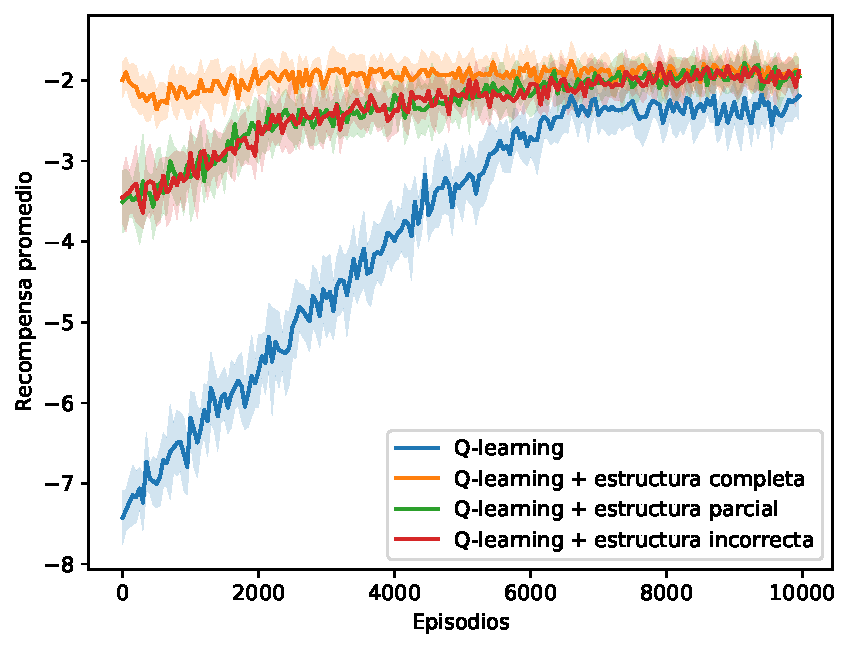
\includegraphics[width=.32\linewidth]{Chapter5/Figs/modexp/deterministic_low_025_one_to_one_N_5_experiments_10_episodes_10000_eps_25000.pdf}&
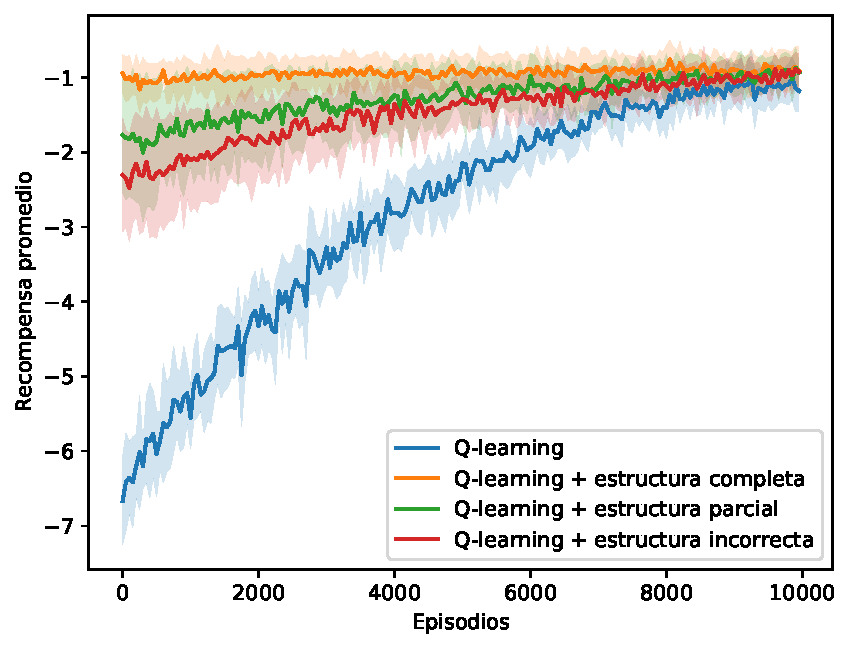
\includegraphics[width=.32\linewidth]{Chapter5/Figs/modexp/deterministic_low_025_one_to_many_N_5_experiments_10_episodes_10000_eps_25000.pdf}&
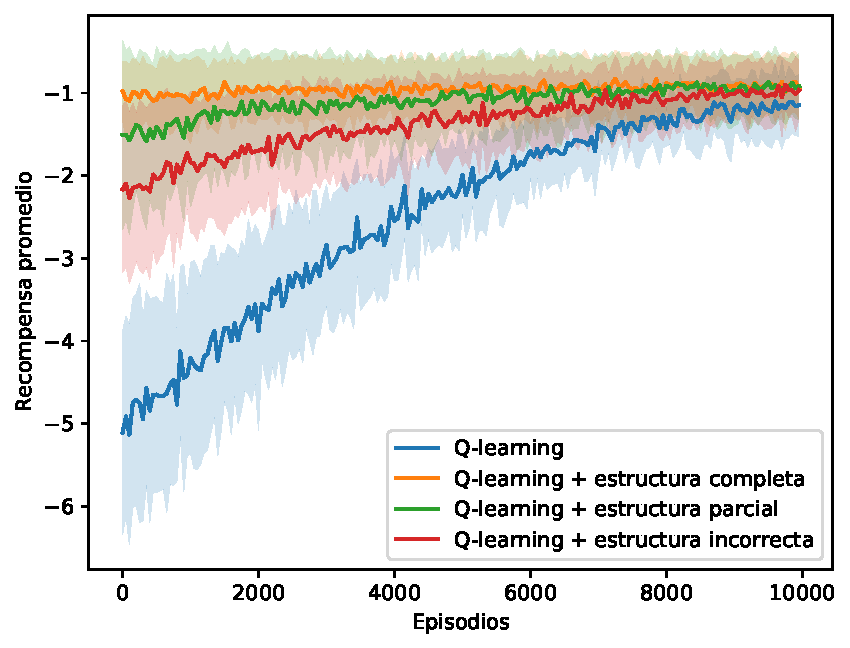
\includegraphics[width=.32\linewidth]{Chapter5/Figs/modexp/deterministic_low_025_many_to_one_N_5_experiments_10_episodes_10000_eps_25000.pdf}
\\
\rowname{$N=7$}&
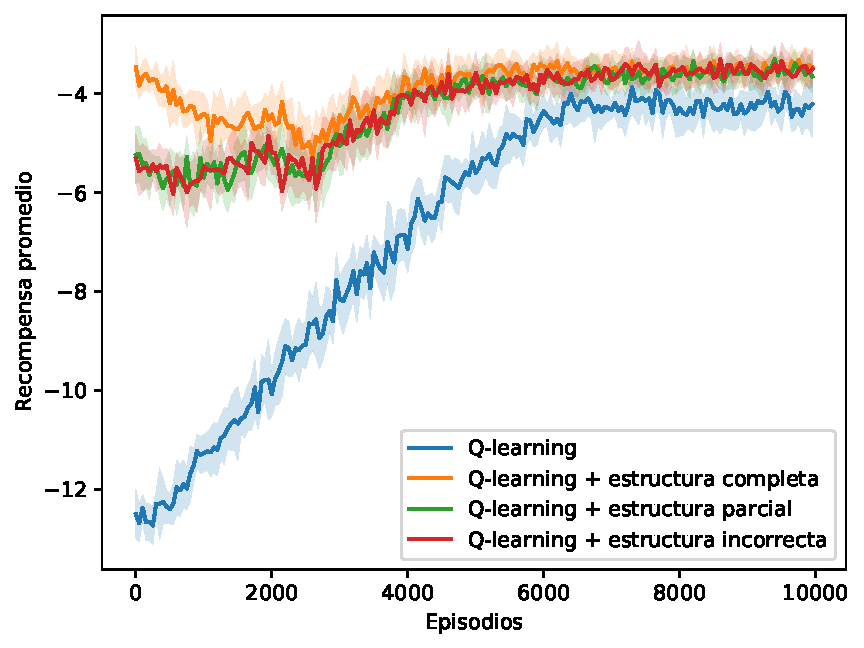
\includegraphics[width=.32\linewidth]{Chapter5/Figs/modexp/deterministic_low_025_one_to_one_N_7_experiments_10_episodes_10000_eps_35000.pdf}&
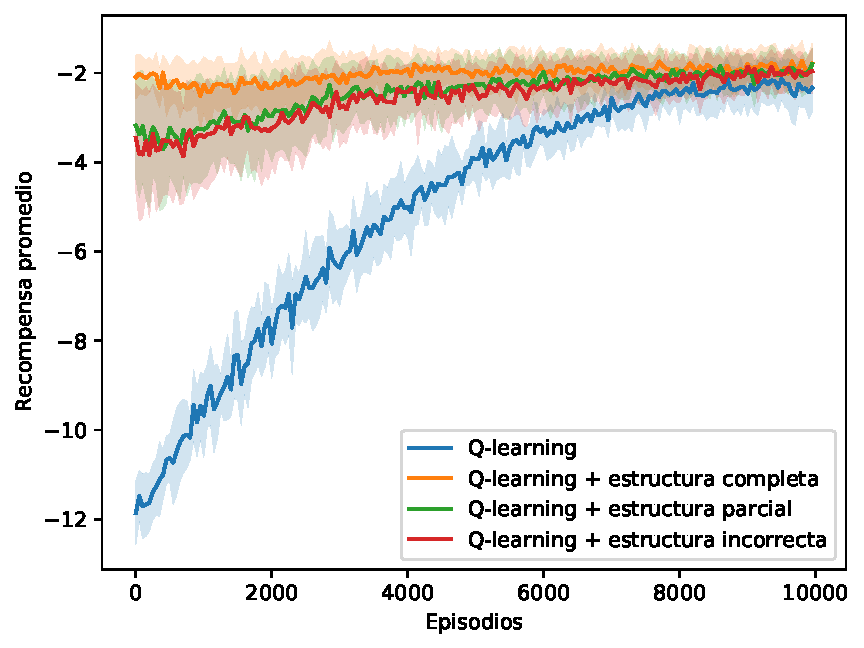
\includegraphics[width=.32\linewidth]{Chapter5/Figs/modexp/deterministic_low_025_one_to_many_N_7_experiments_10_episodes_10000_eps_35000.pdf}&
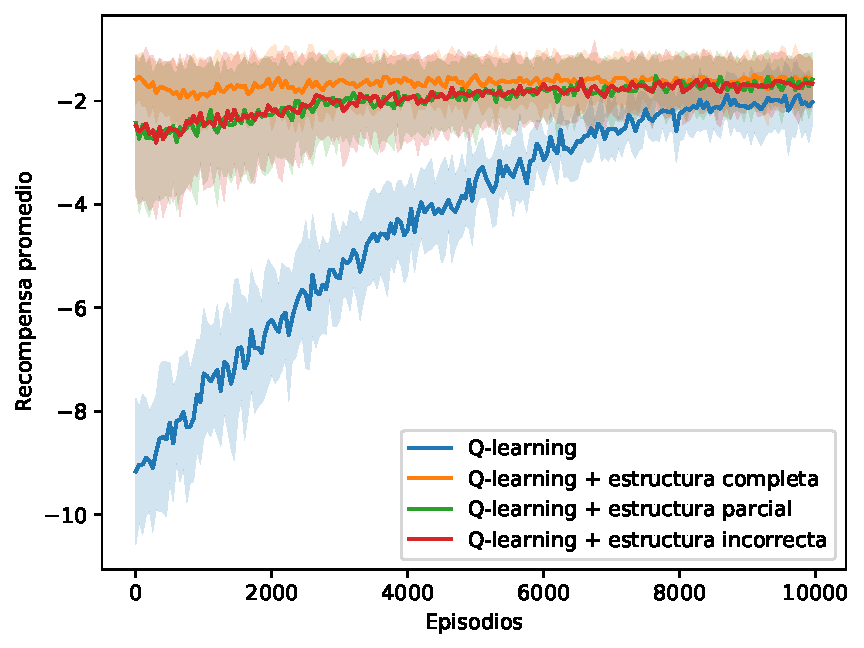
\includegraphics[width=.32\linewidth]{Chapter5/Figs/modexp/deterministic_low_025_many_to_one_N_7_experiments_10_episodes_10000_eps_35000.pdf}
\\
\rowname{$N = 9$}&

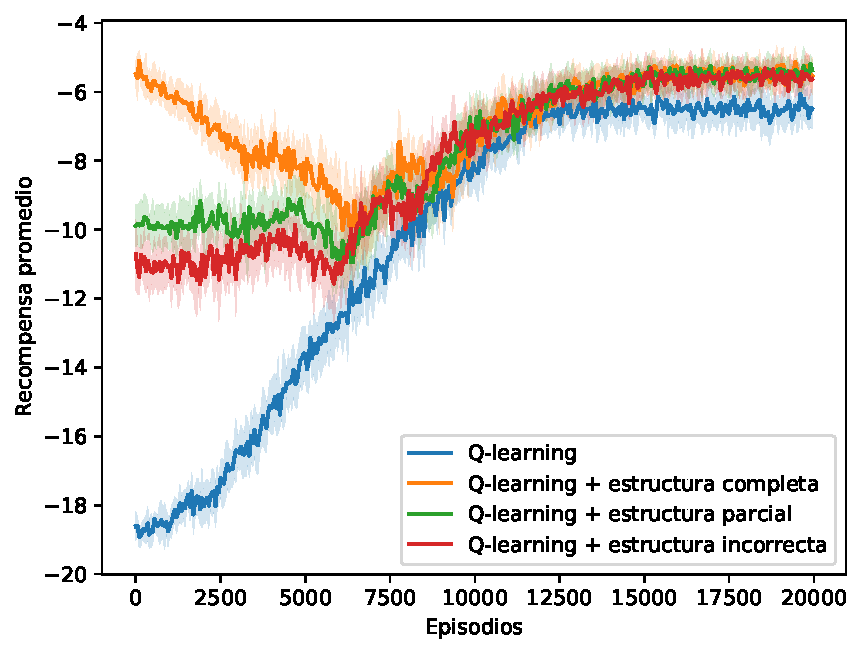
\includegraphics[width=.32\linewidth]{Chapter5/Figs/modexp/deterministic_low_025_one_to_one_N_9_experiments_10_episodes_20000_eps_90000.pdf}&
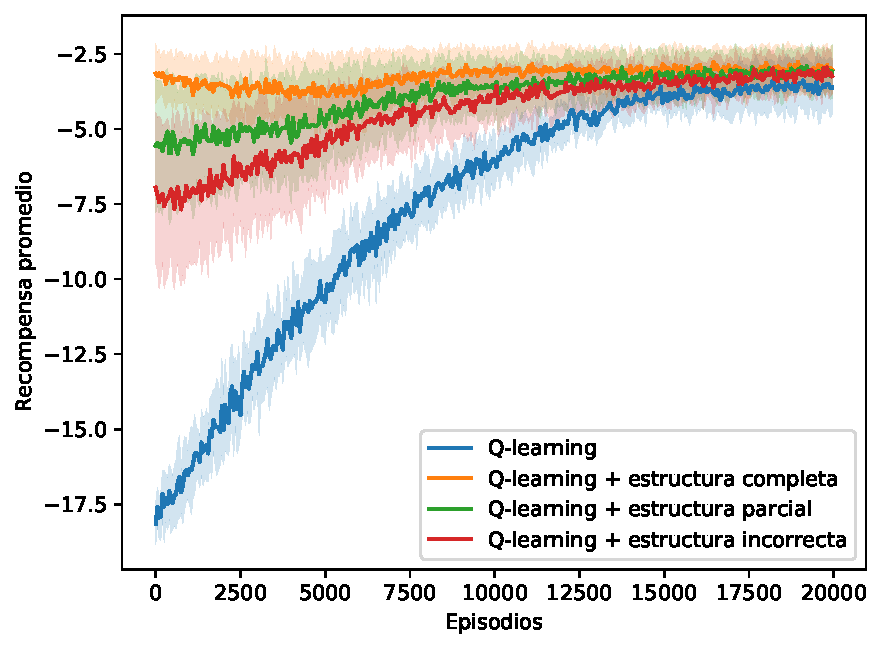
\includegraphics[width=.32\linewidth]{Chapter5/Figs/modexp/deterministic_low_025_one_to_many_N_9_experiments_10_episodes_20000_eps_90000.pdf}&
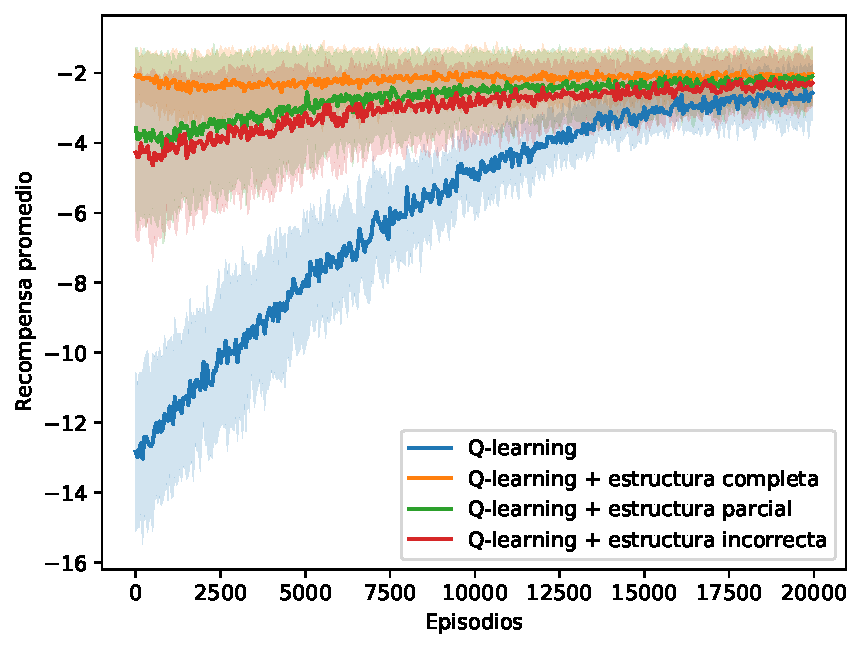
\includegraphics[width=.32\linewidth]{Chapter5/Figs/modexp/deterministic_low_025_many_to_one_N_9_experiments_10_episodes_20000_eps_90000.pdf}

\end{tabular}
\caption{Comparación del desempeño para los 4 algoritmos con un nivel de alteración $p_{mod} = 25 \%$ en un ambiente determinista. Las gráficas muestran la medida $average$ y la desviación estándar (región sombreada) para 10 experimentos con 10000 (para $N = 5, 7$) y 20000 (para $N = 9$) episodios.}
\label{fig:low-mod-det}
\end{figure}

%%%%%%%%%%%%%%%%%
%%%PMOD 25 STO%%%
%%%%%%%%%%%%%%%%%
\begin{figure}
\settoheight{\tempdima}{\includegraphics[width=.32\linewidth]{example-image-a}}%
\centering\begin{tabular}{@{}c@{ }c@{ }c@{ }c@{}}
&\textbf{Uno-a-uno} & \textbf{Causa común} & \textbf{Efecto común} \\
\rowname{$N = 5$}&
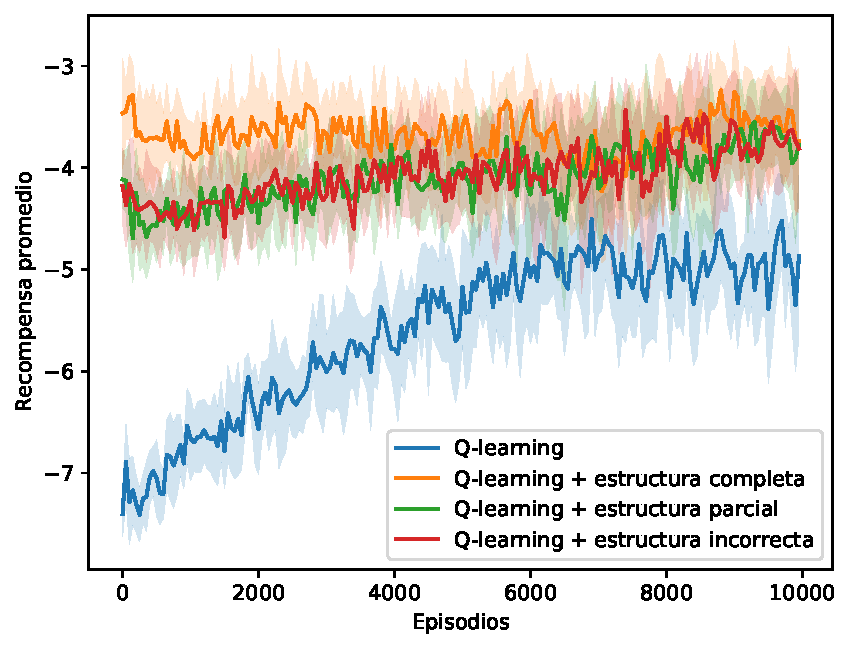
\includegraphics[width=.32\linewidth]{Chapter5/Figs/modexp/stochastic_low_025_one_to_one_N_5_experiments_10_episodes_10000_eps_25000.pdf}&
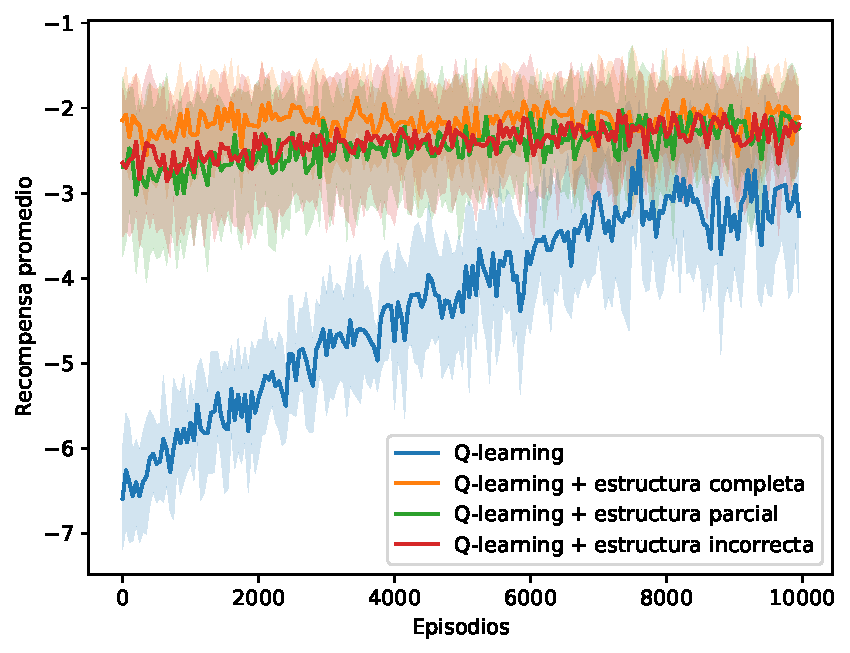
\includegraphics[width=.32\linewidth]{Chapter5/Figs/modexp/stochastic_low_025_one_to_many_N_5_experiments_10_episodes_10000_eps_25000.pdf}&
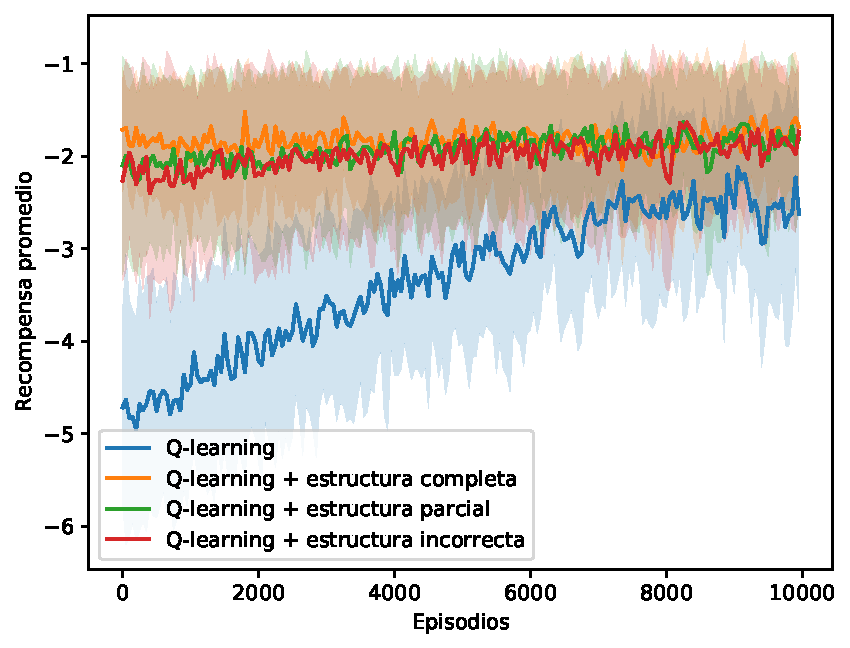
\includegraphics[width=.32\linewidth]{Chapter5/Figs/modexp/stochastic_low_025_many_to_one_N_5_experiments_10_episodes_10000_eps_25000.pdf}
\\
\rowname{$N=7$}&
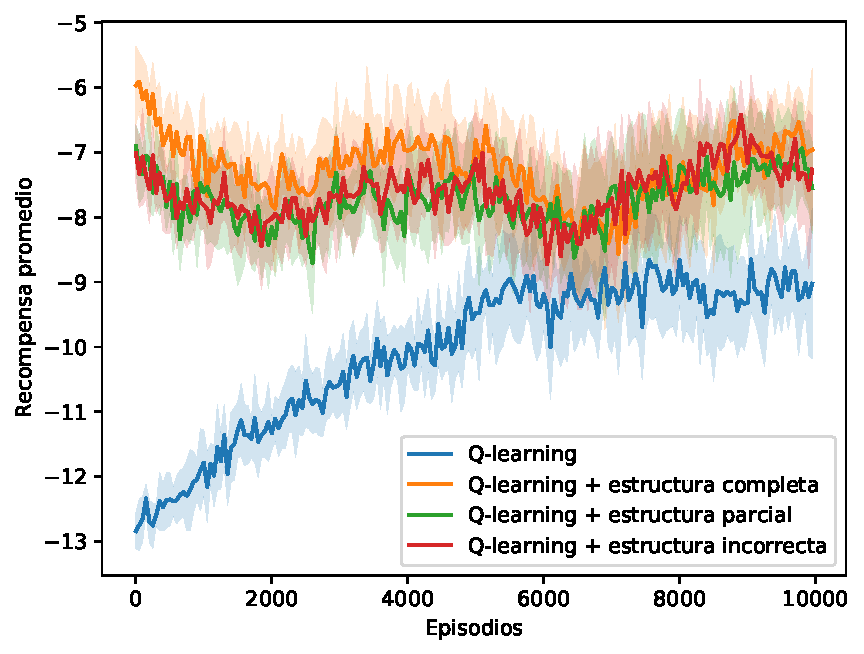
\includegraphics[width=.32\linewidth]{Chapter5/Figs/modexp/stochastic_low_025_one_to_one_N_7_experiments_10_episodes_10000_eps_35000.pdf}&
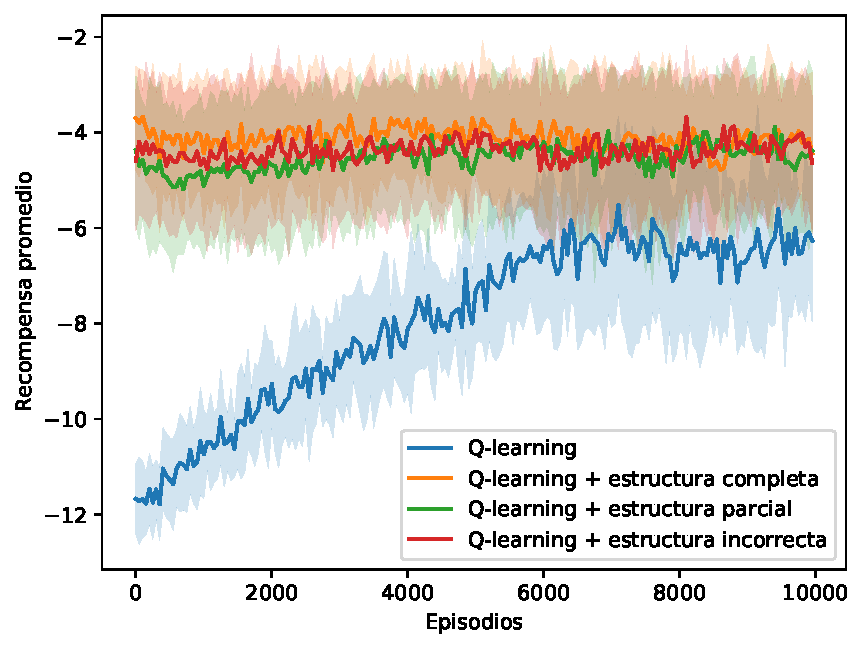
\includegraphics[width=.32\linewidth]{Chapter5/Figs/modexp/stochastic_low_025_one_to_many_N_7_experiments_10_episodes_10000_eps_35000.pdf}&
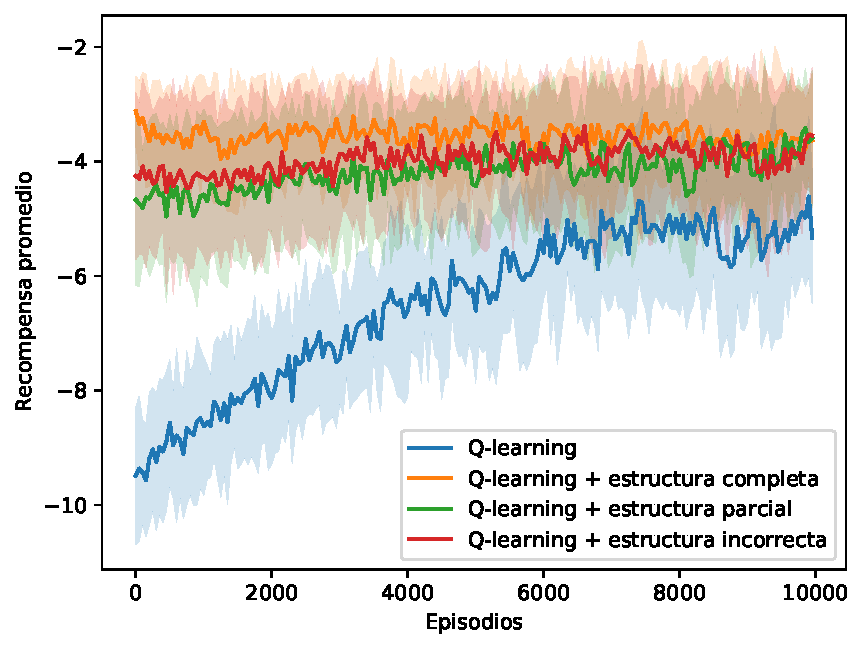
\includegraphics[width=.32\linewidth]{Chapter5/Figs/modexp/stochastic_low_025_many_to_one_N_7_experiments_10_episodes_10000_eps_35000.pdf}
\\
\rowname{$N = 9$}&

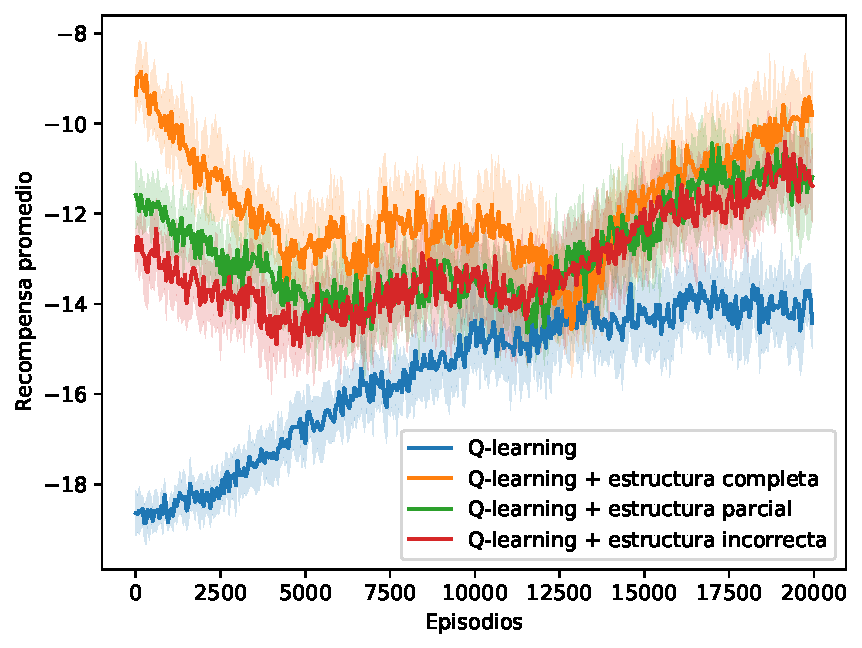
\includegraphics[width=.32\linewidth]{Chapter5/Figs/modexp/stochastic_low_025_one_to_one_N_9_experiments_10_episodes_20000_eps_90000.pdf}&
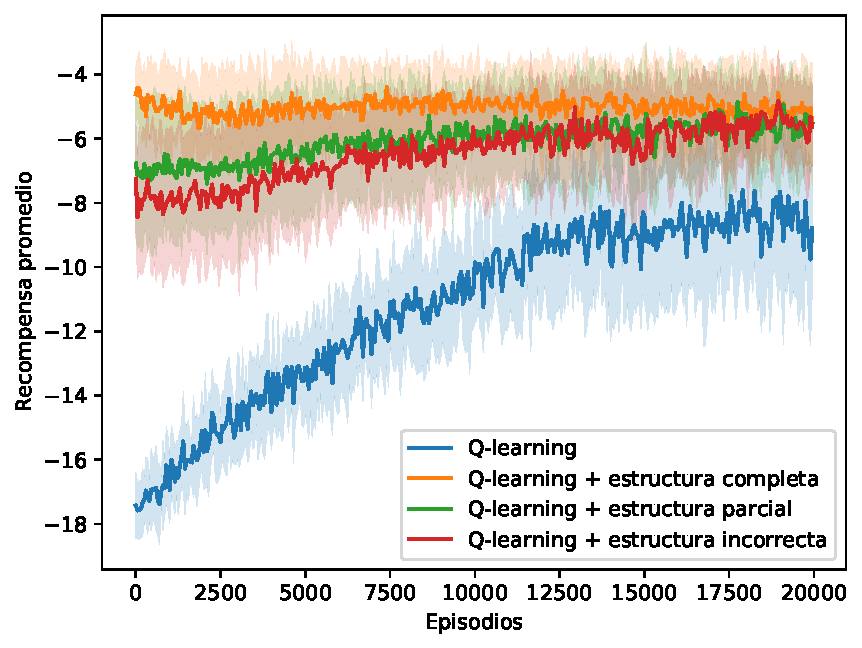
\includegraphics[width=.32\linewidth]{Chapter5/Figs/modexp/stochastic_low_025_one_to_many_N_9_experiments_10_episodes_20000_eps_90000.pdf}&
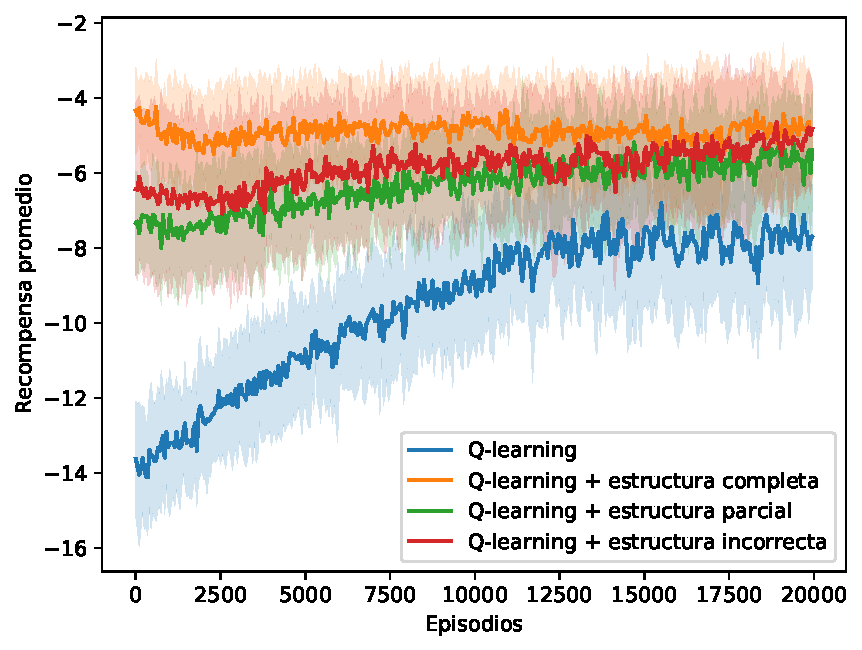
\includegraphics[width=.32\linewidth]{Chapter5/Figs/modexp/stochastic_low_025_many_to_one_N_9_experiments_10_episodes_20000_eps_90000.pdf}

\end{tabular}
\caption{Comparación del desempeño para los 4 algoritmos con un nivel de alteración $p_{mod} = 25 \%$ en un ambiente estocástico. Las gráficas muestran la medida $average$ y la desviación estándar (región sombreada) para 10 experimentos con 10000 (para $N = 5, 7$) y 20000 (para $N = 9$) episodios.}
\label{fig:low-mod-sto}
\end{figure}


\begin{figure}
\settoheight{\tempdima}{\includegraphics[width=.32\linewidth]{example-image-a}}%
\centering\begin{tabular}{@{}c@{ }c@{ }c@{ }c@{}}
&\textbf{Uno-a-uno} & \textbf{Causa común} & \textbf{Efecto común} \\
\rowname{$N = 5$}&
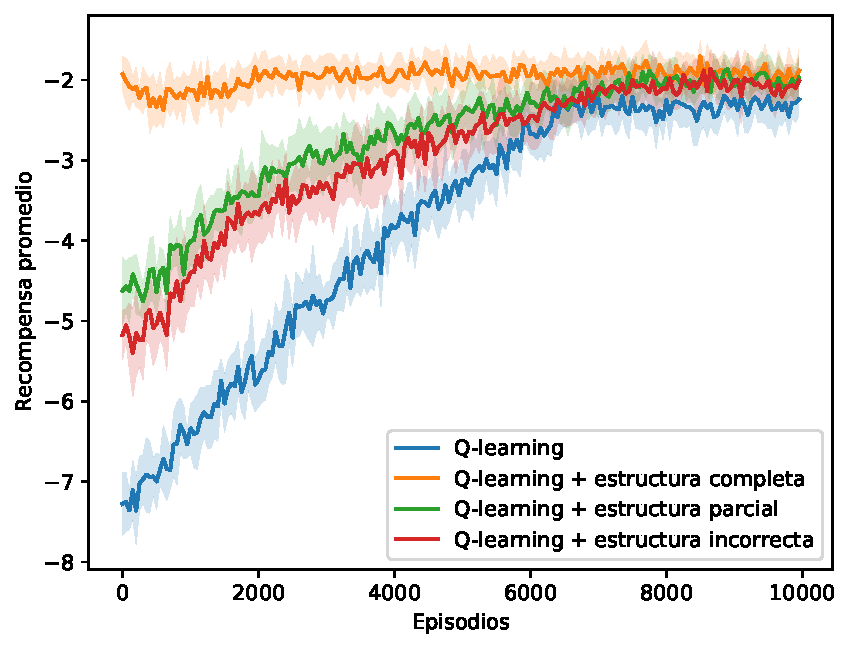
\includegraphics[width=.32\linewidth]{Chapter5/Figs/modexp/deterministic_medium_05_one_to_one_N_5_experiments_10_episodes_10000_eps_25000.pdf}&
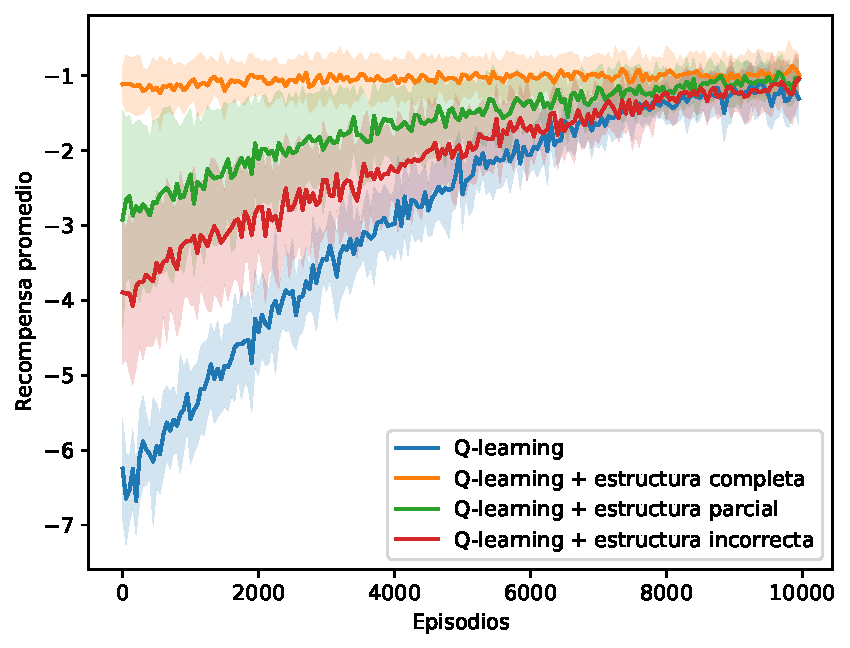
\includegraphics[width=.32\linewidth]{Chapter5/Figs/modexp/deterministic_medium_05_one_to_many_N_5_experiments_10_episodes_10000_eps_25000.pdf}&
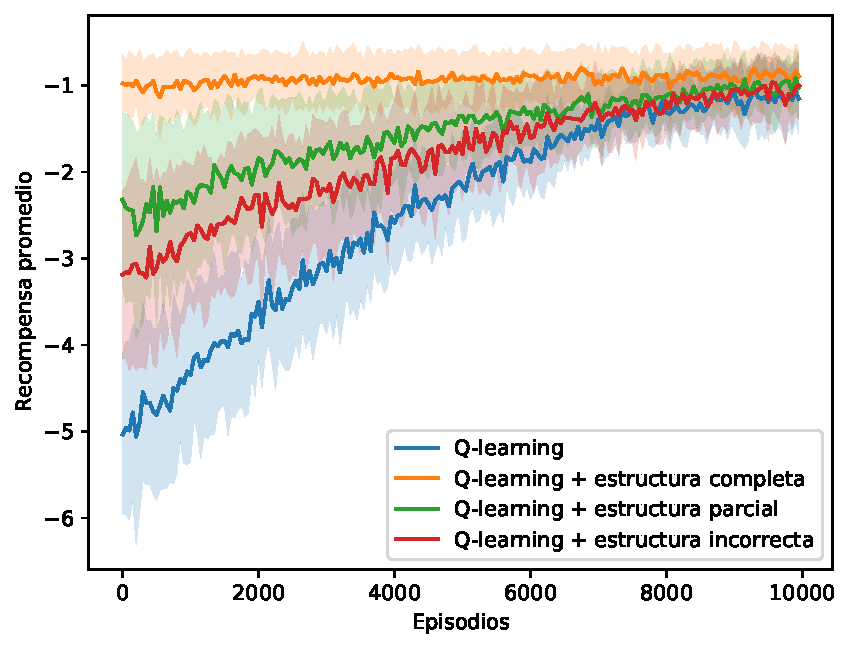
\includegraphics[width=.32\linewidth]{Chapter5/Figs/modexp/deterministic_medium_05_many_to_one_N_5_experiments_10_episodes_10000_eps_25000.pdf}
\\
\rowname{$N=7$}&
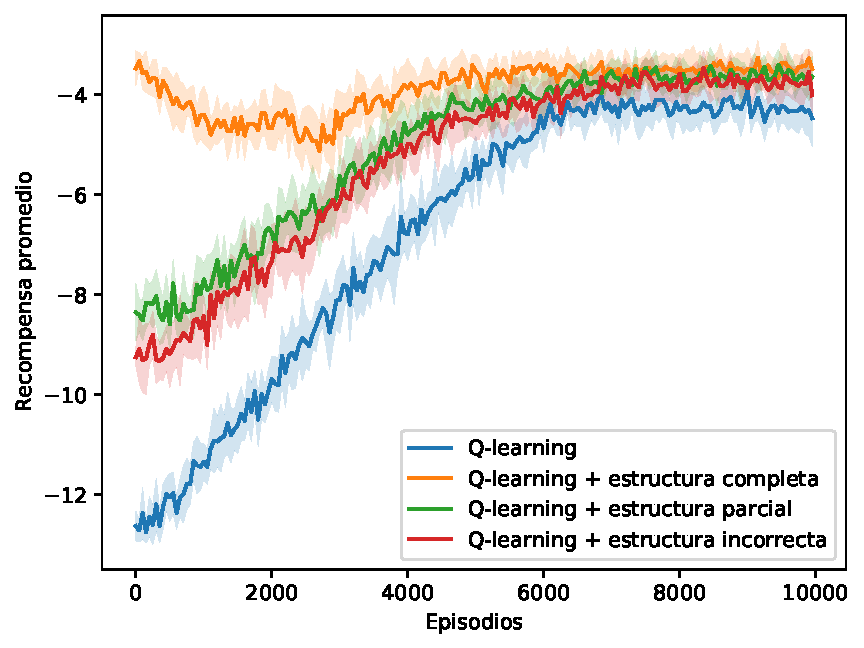
\includegraphics[width=.32\linewidth]{Chapter5/Figs/modexp/deterministic_medium_05_one_to_one_N_7_experiments_10_episodes_10000_eps_35000.pdf}&
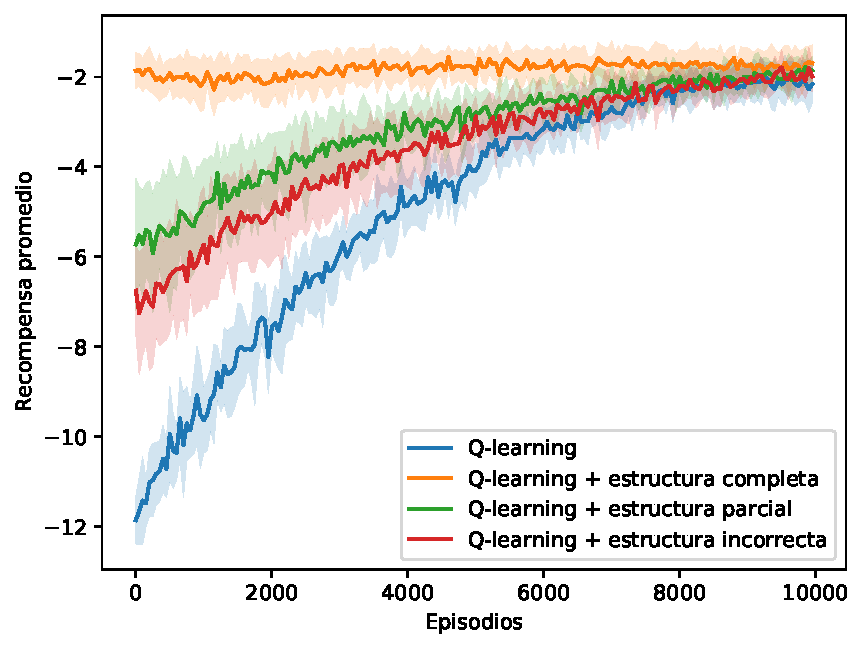
\includegraphics[width=.32\linewidth]{Chapter5/Figs/modexp/deterministic_medium_05_one_to_many_N_7_experiments_10_episodes_10000_eps_35000.pdf}&
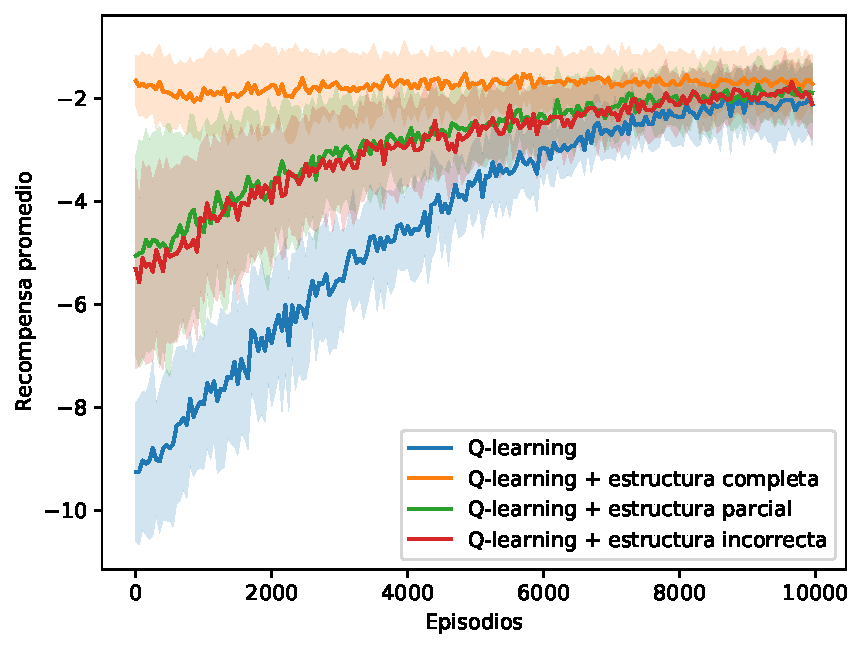
\includegraphics[width=.32\linewidth]{Chapter5/Figs/modexp/deterministic_medium_05_many_to_one_N_7_experiments_10_episodes_10000_eps_35000.pdf}
\\
\rowname{$N = 9$}&

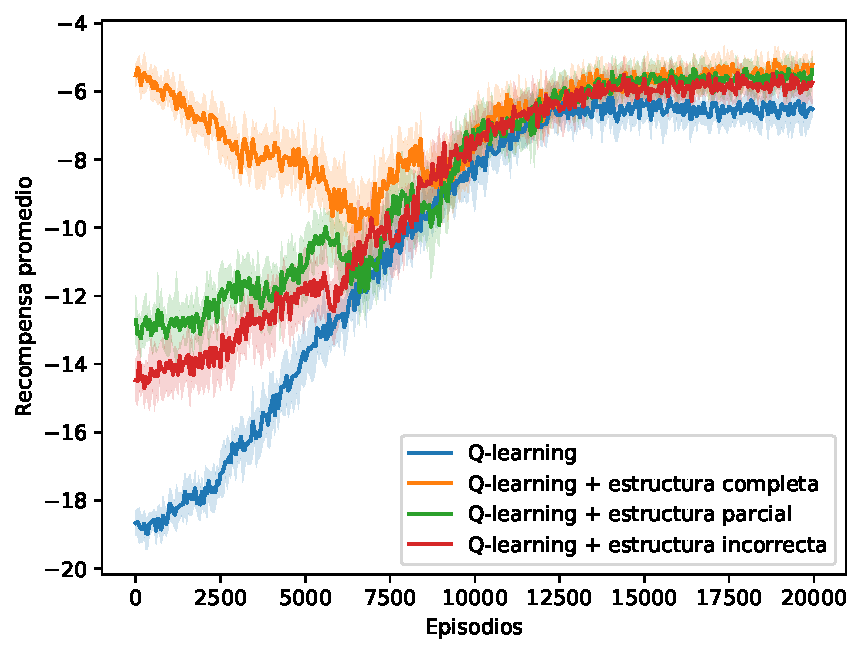
\includegraphics[width=.32\linewidth]{Chapter5/Figs/modexp/deterministic_medium_05_one_to_one_N_9_experiments_10_episodes_20000_eps_90000.pdf}&
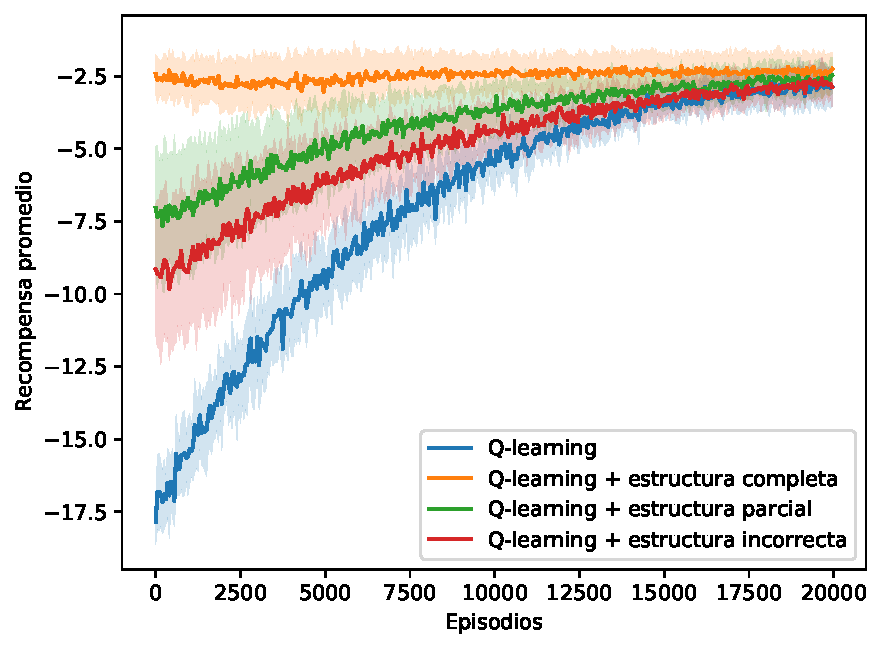
\includegraphics[width=.32\linewidth]{Chapter5/Figs/modexp/deterministic_medium_05_one_to_many_N_9_experiments_10_episodes_20000_eps_90000.pdf}&
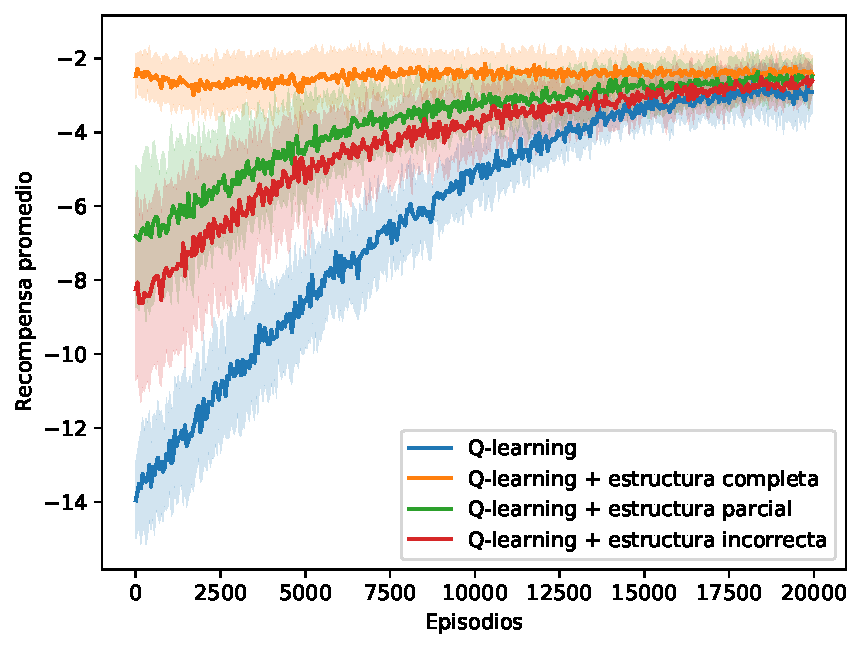
\includegraphics[width=.32\linewidth]{Chapter5/Figs/modexp/deterministic_medium_05_many_to_one_N_9_experiments_10_episodes_20000_eps_90000.pdf}

\end{tabular}
\caption{Comparación del desempeño para los 4 algoritmos con un nivel de alteración $p_{mod} = 50 \%$ en un ambiente determinista. Las gráficas muestran la medida $average$ y la desviación estándar (región sombreada)para 10 experimentos con 10000 (para $N = 5, 7$) y 20000 (para $N = 9$) episodios.}
\label{fig:med-mod-det}
\end{figure}



\begin{figure}
\settoheight{\tempdima}{\includegraphics[width=.32\linewidth]{example-image-a}}%
\centering\begin{tabular}{@{}c@{ }c@{ }c@{ }c@{}}
&\textbf{Uno-a-uno} & \textbf{Causa común} & \textbf{Efecto común} \\
\rowname{$N = 5$}&
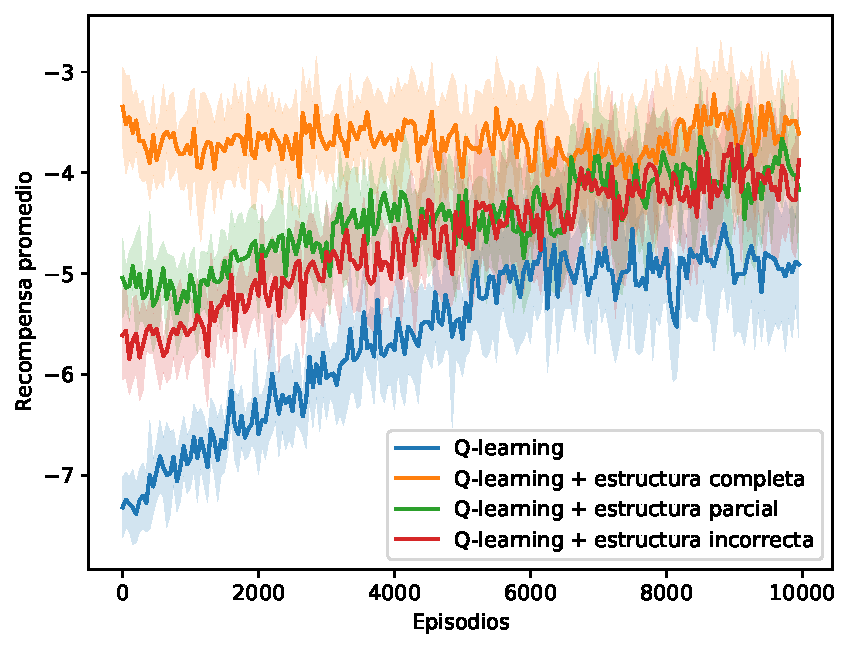
\includegraphics[width=.32\linewidth]{Chapter5/Figs/modexp/stochastic_medium_05_one_to_one_N_5_experiments_10_episodes_10000_eps_25000.pdf}&
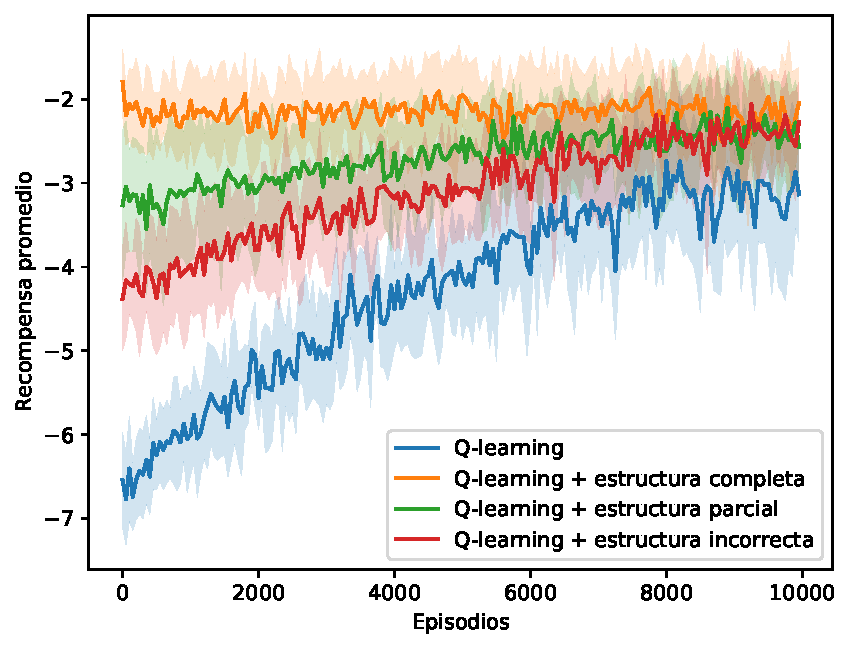
\includegraphics[width=.32\linewidth]{Chapter5/Figs/modexp/stochastic_medium_05_one_to_many_N_5_experiments_10_episodes_10000_eps_25000.pdf}&
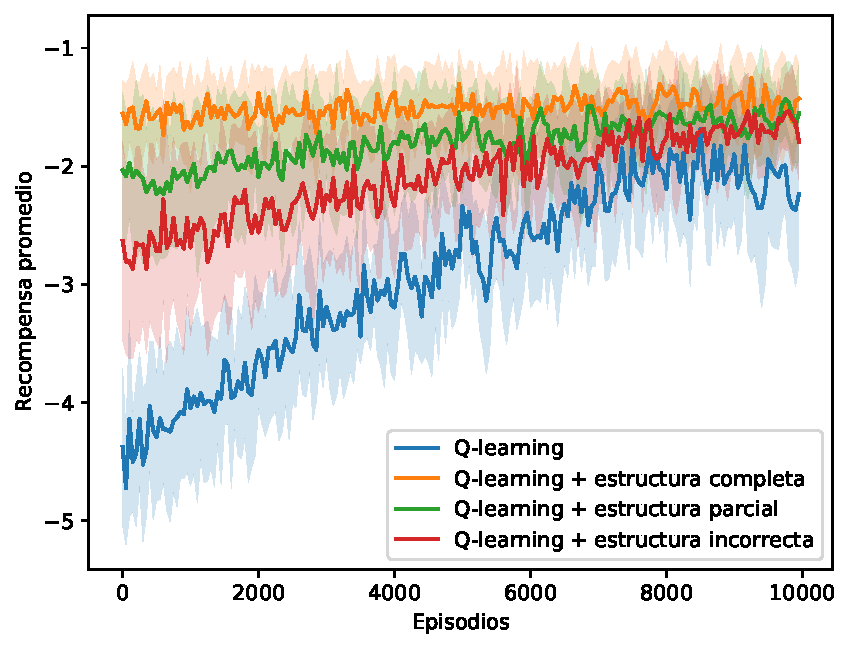
\includegraphics[width=.32\linewidth]{Chapter5/Figs/modexp/stochastic_medium_05_many_to_one_N_5_experiments_10_episodes_10000_eps_25000.pdf}
\\
\rowname{$N=7$}&
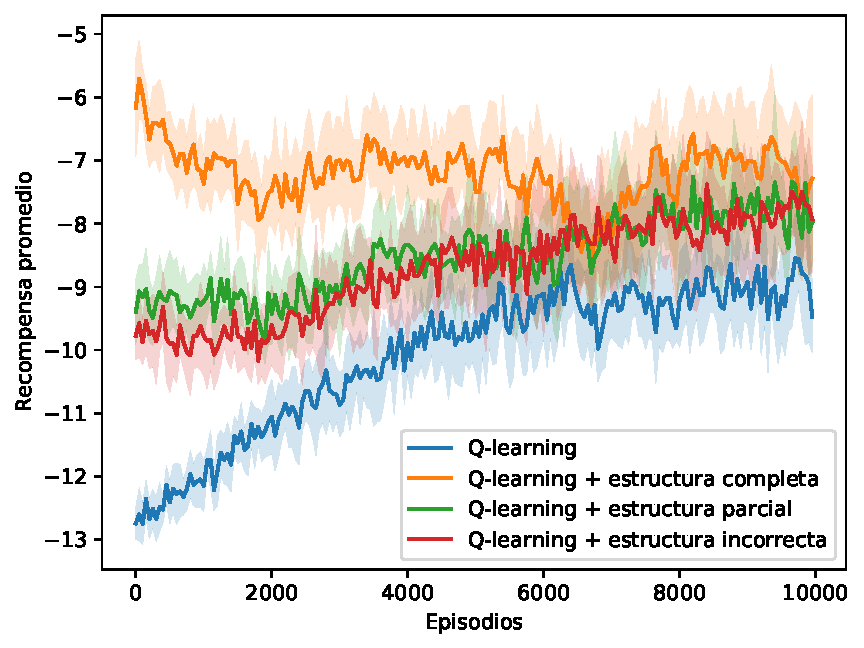
\includegraphics[width=.32\linewidth]{Chapter5/Figs/modexp/stochastic_medium_05_one_to_one_N_7_experiments_10_episodes_10000_eps_35000.pdf}&
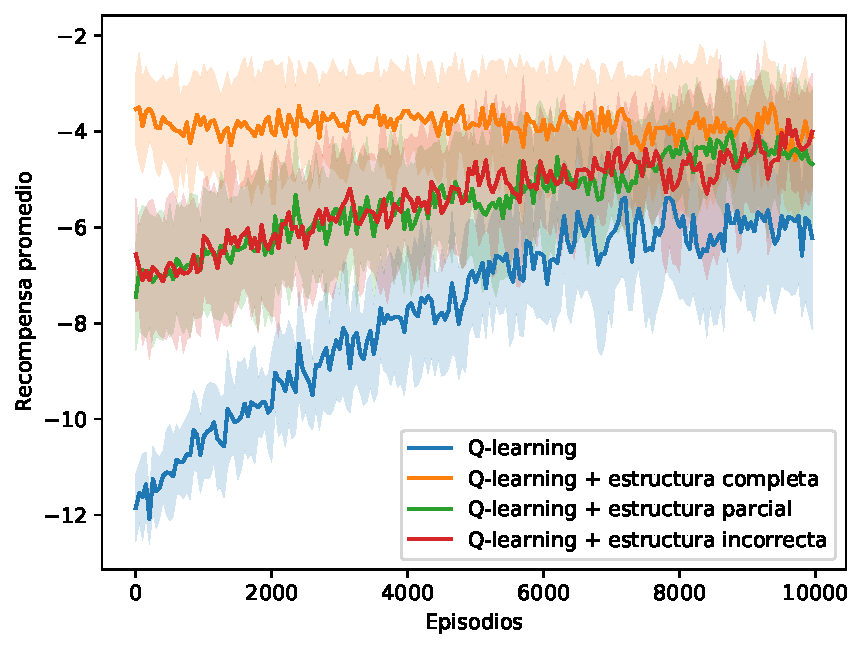
\includegraphics[width=.32\linewidth]{Chapter5/Figs/modexp/stochastic_medium_05_one_to_many_N_7_experiments_10_episodes_10000_eps_35000.pdf}&
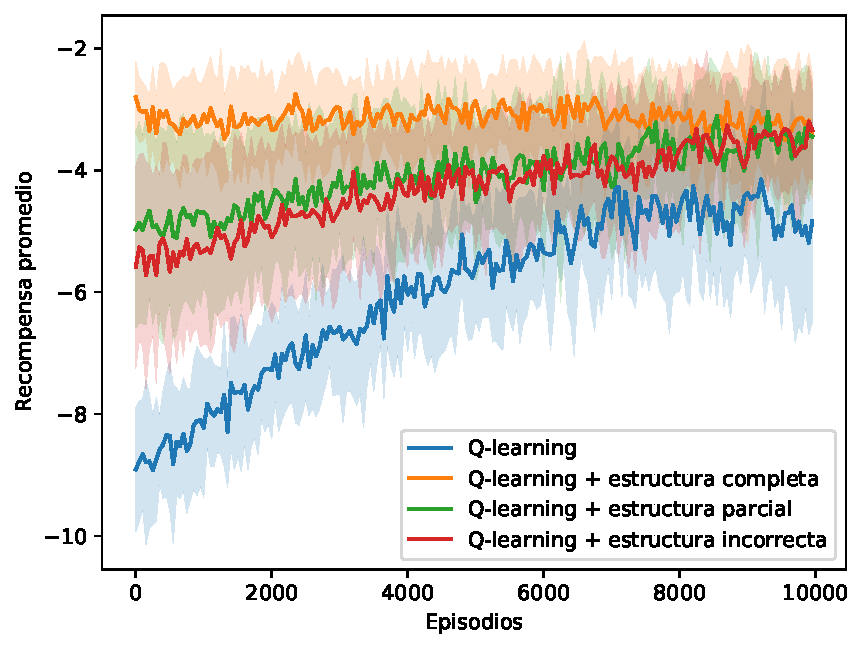
\includegraphics[width=.32\linewidth]{Chapter5/Figs/modexp/stochastic_medium_05_many_to_one_N_7_experiments_10_episodes_10000_eps_35000.pdf}
\\
\rowname{$N = 9$}&

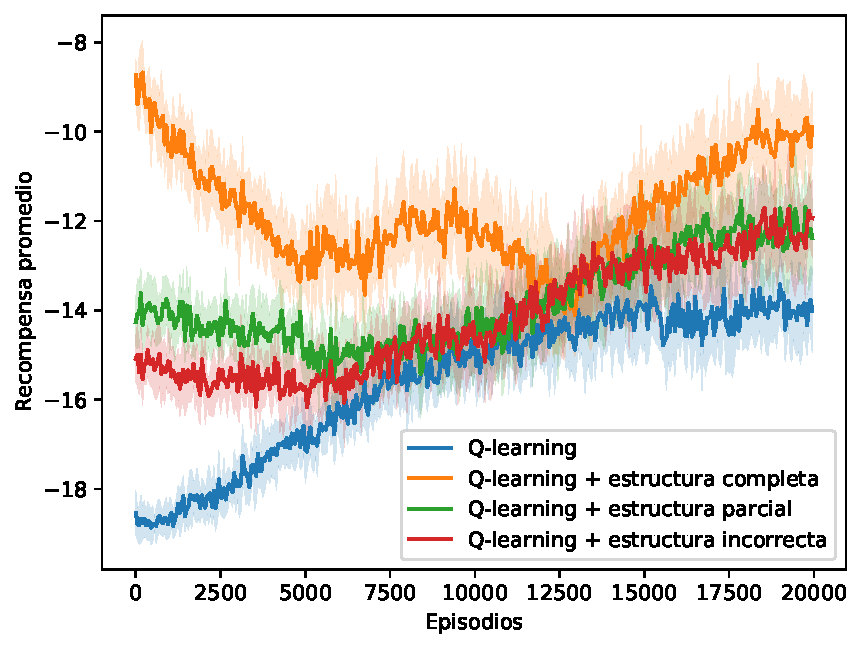
\includegraphics[width=.32\linewidth]{Chapter5/Figs/modexp/stochastic_medium_05_one_to_one_N_9_experiments_10_episodes_20000_eps_90000.pdf}&
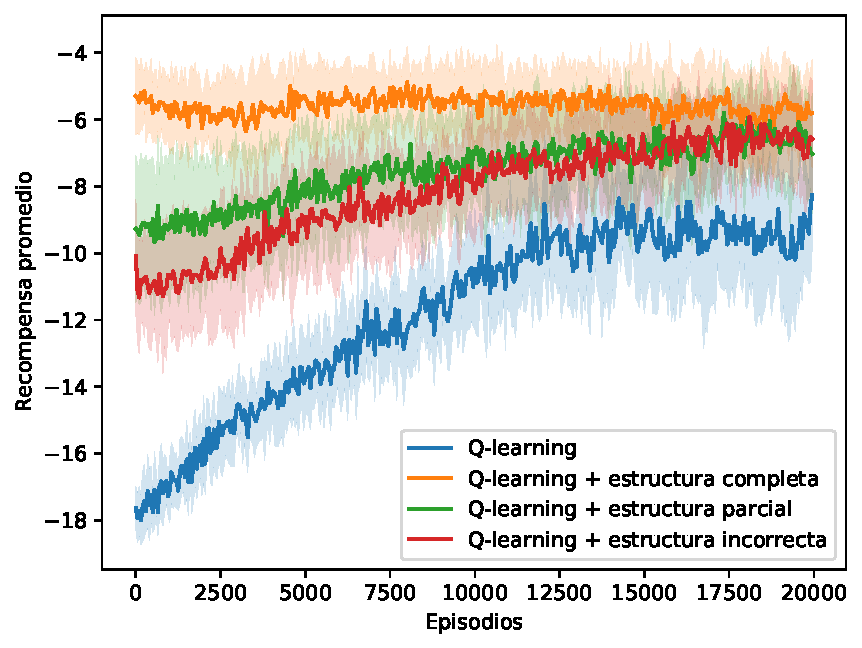
\includegraphics[width=.32\linewidth]{Chapter5/Figs/modexp/stochastic_medium_05_one_to_many_N_9_experiments_10_episodes_20000_eps_90000.pdf}&
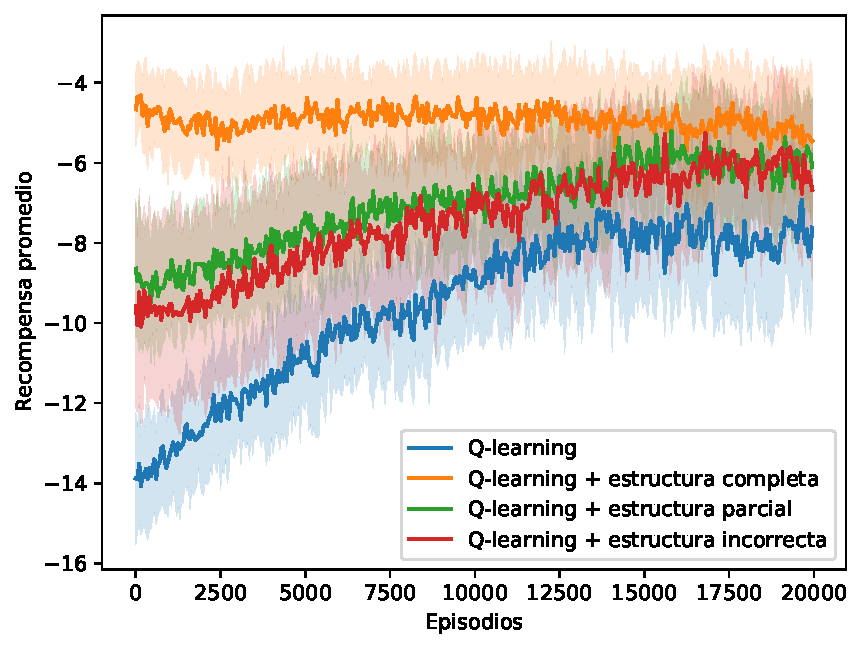
\includegraphics[width=.32\linewidth]{Chapter5/Figs/modexp/stochastic_medium_05_many_to_one_N_9_experiments_10_episodes_20000_eps_90000.pdf}

\end{tabular}
\caption{Comparación del desempeño para los 4 algoritmos con un nivel de alteración $p_{mod} = 50 \%$ en un ambiente estocástico. Las gráficas muestran la medida $average$ y la desviación estándar (región sombreada)para 10 experimentos con 10000 (para $N = 5, 7$) y 20000 (para $N = 9$) episodios.}
\label{fig:med-mod-sto}
\end{figure}



\begin{figure}
\settoheight{\tempdima}{\includegraphics[width=.32\linewidth]{example-image-a}}%
\centering\begin{tabular}{@{}c@{ }c@{ }c@{ }c@{}}
&\textbf{Uno-a-uno} & \textbf{Causa común} & \textbf{Efecto común} \\
\rowname{$N = 5$}&
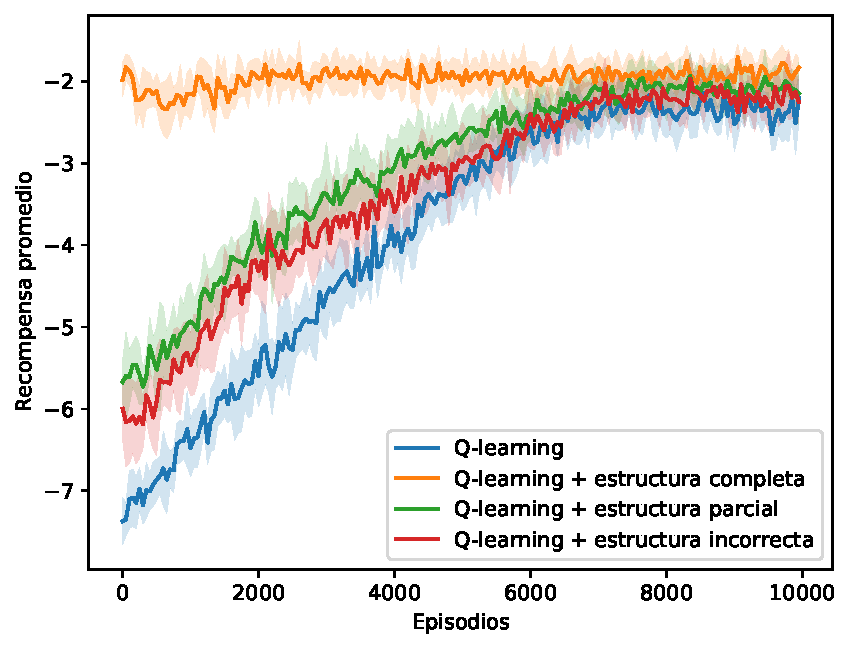
\includegraphics[width=.32\linewidth]{Chapter5/Figs/modexp/deterministic_high_075_one_to_one_N_5_experiments_10_episodes_10000_eps_25000.pdf}&
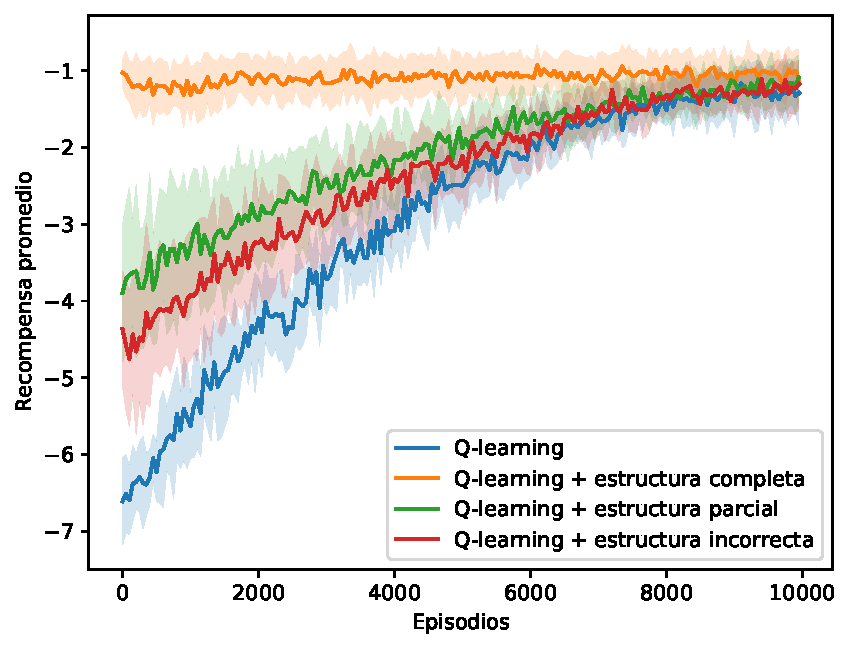
\includegraphics[width=.32\linewidth]{Chapter5/Figs/modexp/deterministic_high_075_one_to_many_N_5_experiments_10_episodes_10000_eps_25000.pdf}&
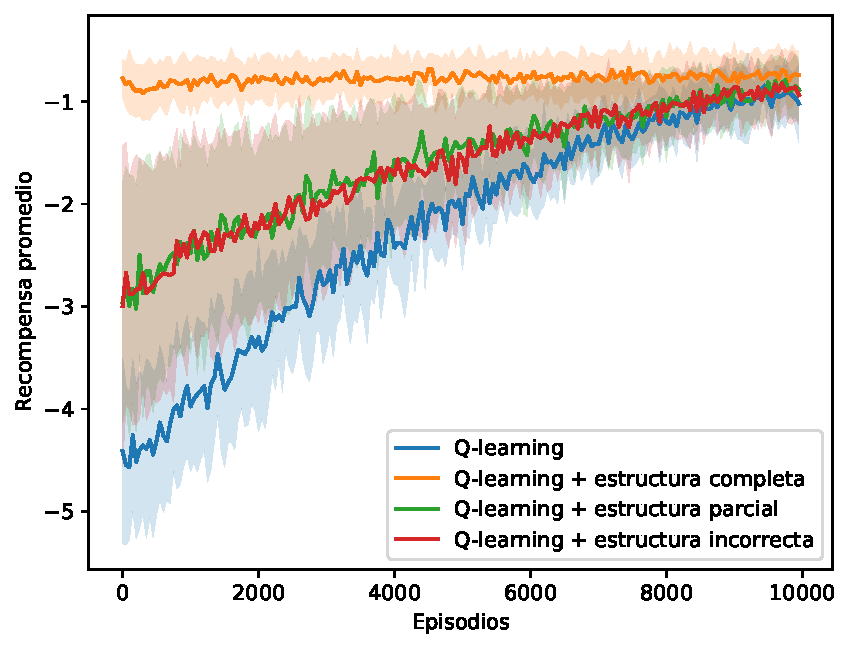
\includegraphics[width=.32\linewidth]{Chapter5/Figs/modexp/deterministic_high_075_many_to_one_N_5_experiments_10_episodes_10000_eps_25000.pdf}
\\
\rowname{$N=7$}&
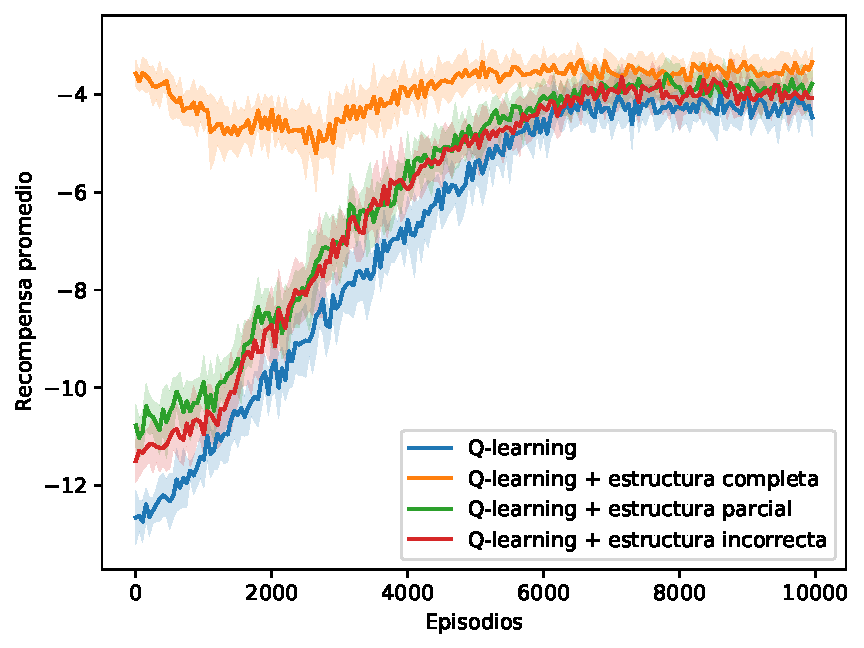
\includegraphics[width=.32\linewidth]{Chapter5/Figs/modexp/deterministic_high_075_one_to_one_N_7_experiments_10_episodes_10000_eps_35000.pdf}&
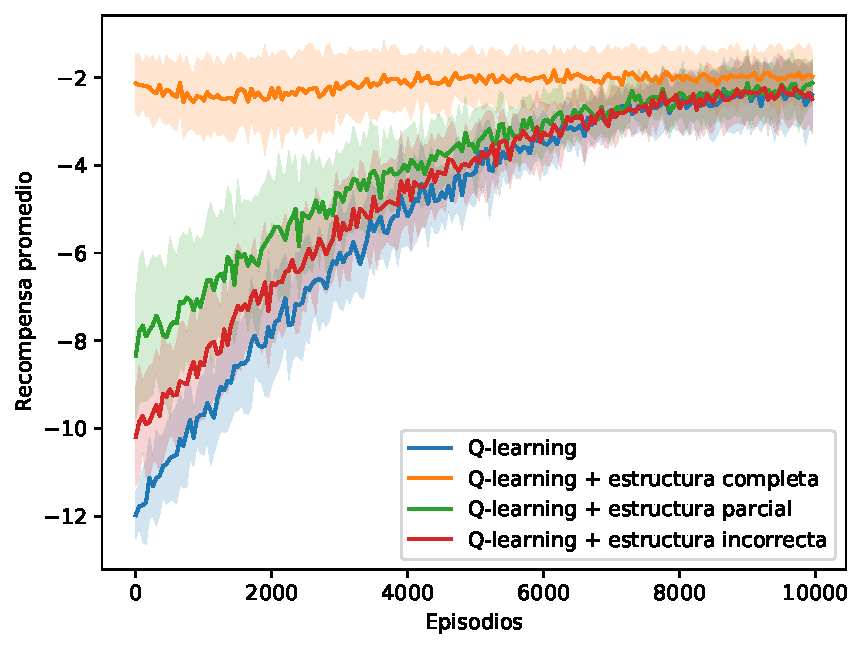
\includegraphics[width=.32\linewidth]{Chapter5/Figs/modexp/deterministic_high_075_one_to_many_N_7_experiments_10_episodes_10000_eps_35000.pdf}&
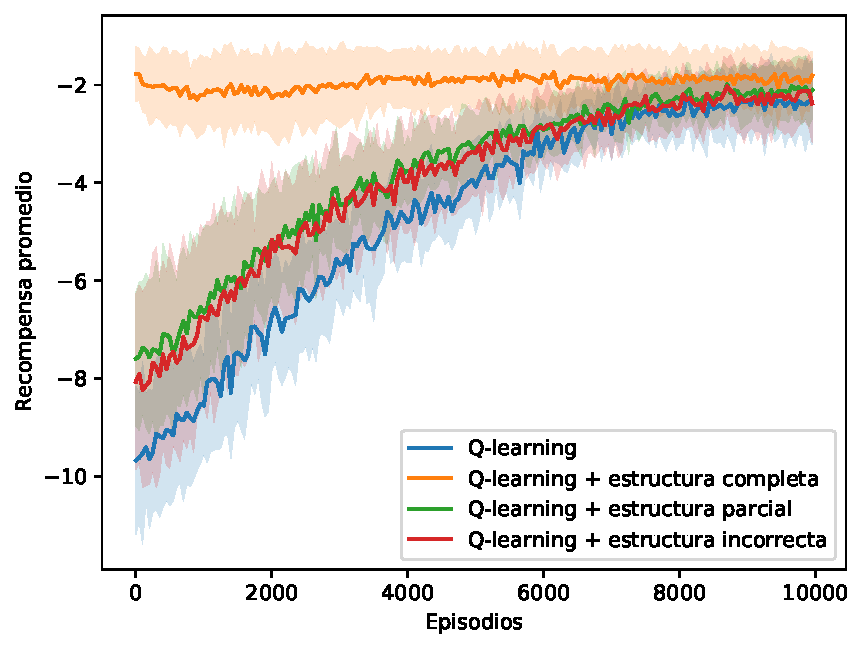
\includegraphics[width=.32\linewidth]{Chapter5/Figs/modexp/deterministic_high_075_many_to_one_N_7_experiments_10_episodes_10000_eps_35000.pdf}
\\
\rowname{$N = 9$}&

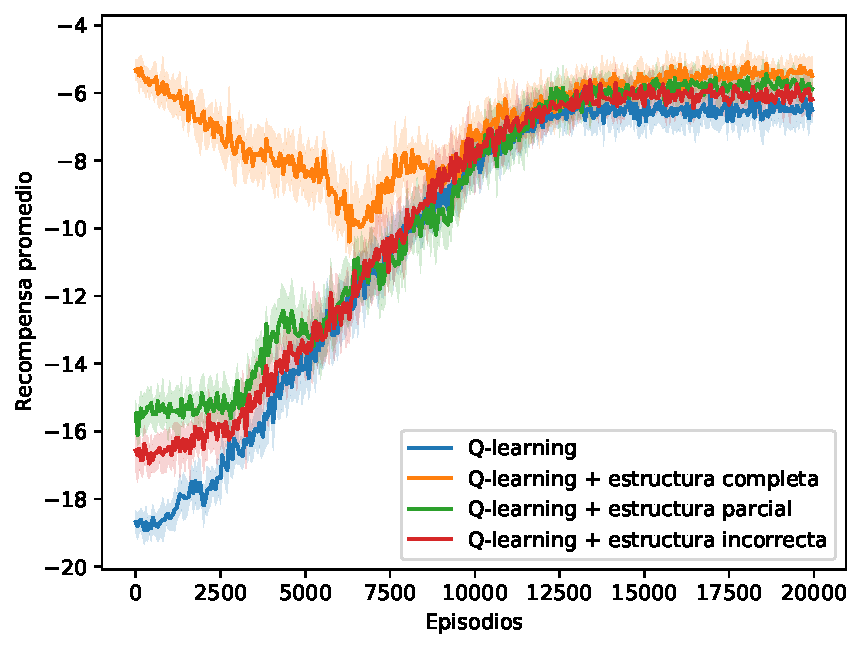
\includegraphics[width=.32\linewidth]{Chapter5/Figs/modexp/deterministic_high_075_one_to_one_N_9_experiments_10_episodes_20000_eps_90000.pdf}&
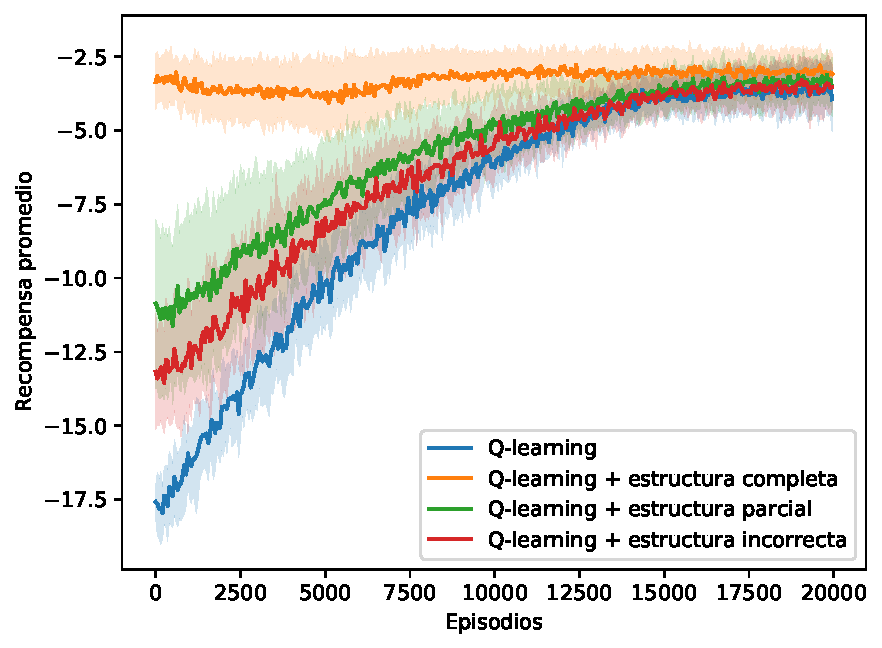
\includegraphics[width=.32\linewidth]{Chapter5/Figs/modexp/deterministic_high_075_one_to_many_N_9_experiments_10_episodes_20000_eps_90000.pdf}&
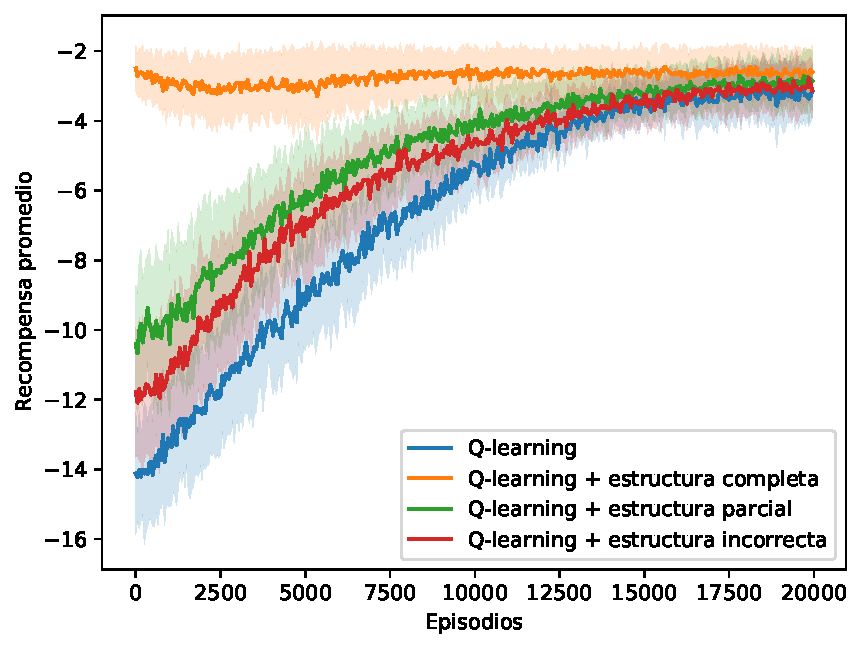
\includegraphics[width=.32\linewidth]{Chapter5/Figs/modexp/deterministic_high_075_many_to_one_N_9_experiments_10_episodes_20000_eps_90000.pdf}


\end{tabular}

\caption{Comparación del desempeño para los 4 algoritmos con un nivel de alteración $p_{mod} = 75 \%$ en un ambiente determinista. Las gráficas muestran la medida $average$ y la desviación estándar (región sombreada) para 10 experimentos con 10000 (para $N = 5, 7$) y 20000 (para $N = 9$) episodios.}
\label{fig:high-mod-det}
\end{figure}

\begin{figure}
\settoheight{\tempdima}{\includegraphics[width=.32\linewidth]{example-image-a}}%
\centering\begin{tabular}{@{}c@{ }c@{ }c@{ }c@{}}
&\textbf{Uno-a-uno} & \textbf{Causa común} & \textbf{Efecto común} \\
\rowname{$N = 5$}&
\includegraphics[width=.32\linewidth]{Chapter5/Figs/modexp/stochastic_high_075_one_to_one_N_5_experiments_10_episodes_10000_eps_25000.pdf}&
\includegraphics[width=.32\linewidth]{Chapter5/Figs/modexp/stochastic_high_075_one_to_many_N_5_experiments_10_episodes_10000_eps_25000.pdf}&
\includegraphics[width=.32\linewidth]{Chapter5/Figs/modexp/stochastic_high_075_many_to_one_N_5_experiments_10_episodes_10000_eps_25000.pdf}
\\
\rowname{$N=7$}&
\includegraphics[width=.32\linewidth]{Chapter5/Figs/modexp/stochastic_high_075_one_to_one_N_7_experiments_10_episodes_10000_eps_35000.pdf}&
\includegraphics[width=.32\linewidth]{Chapter5/Figs/modexp/stochastic_high_075_one_to_many_N_7_experiments_10_episodes_10000_eps_35000.pdf}&
\includegraphics[width=.32\linewidth]{Chapter5/Figs/modexp/stochastic_high_075_many_to_one_N_7_experiments_10_episodes_10000_eps_35000.pdf}
\\
\rowname{$N = 9$}&

\includegraphics[width=.32\linewidth]{Chapter5/Figs/modexp/stochastic_high_075_one_to_one_N_9_experiments_10_episodes_20000_eps_90000.pdf}&
\includegraphics[width=.32\linewidth]{Chapter5/Figs/modexp/stochastic_high_075_one_to_many_N_9_experiments_10_episodes_20000_eps_90000.pdf}&
\includegraphics[width=.32\linewidth]{Chapter5/Figs/modexp/stochastic_high_075_many_to_one_N_9_experiments_10_episodes_20000_eps_90000.pdf}
\end{tabular}

\caption{Comparación del desempeño para los 4 algoritmos con un nivel de alteración $p_{mod} = 75 \%$ en un ambiente estocástico. Las gráficas muestran la medida $average$ y la desviación estándar (región sombreada) para 10 experimentos con 10000 (para $N = 5, 7$) y 20000 (para $N = 9$) episodios.}
\label{fig:high-mod-sto}
\end{figure}


